\documentclass[twoside,11pt]{article}

\usepackage{blindtext}

% Any additional packages needed should be included after jmlr2e.
% Note that jmlr2e.sty includes epsfig, amssymb, natbib and graphicx,
% and defines many common macros, such as 'proof' and 'example'.
%
% It also sets the bibliographystyle to plainnat; for more information on
% natbib citation styles, see the natbib documentation, a copy of which
% is archived at http://www.jmlr.org/format/natbib.pdf

% Available options for package jmlr2e are:
%
%   - abbrvbib : use abbrvnat for the bibliography style
%   - nohyperref : do not load the hyperref package
%   - preprint : remove JMLR specific information from the template,
%         useful for example for posting to preprint servers.
%
% Example of using the package with custom options:
%
% \usepackage[abbrvbib, preprint]{jmlr2e}

\usepackage{jmlr2e}

% Definitions of handy macros can go here

\newcommand{\dataset}{{\cal D}}
\newcommand{\fracpartial}[2]{\frac{\partial #1}{\partial  #2}}

% Heading arguments are {volume}{year}{pages}{date submitted}{date published}{paper id}{author-full-names}

\usepackage{lastpage}
\jmlrheading{23}{2022}{1-\pageref{LastPage}}{1/21; Revised 5/22}{9/22}{21-0000}{Hao Wang and Ye Wang}

% Short headings should be running head and authors last names

\ShortHeadings{Sample JMLR Paper}{One and Two}
\firstpageno{1}




% \usepackage{svg}
\usepackage[utf8]{inputenc} % allow utf-8 input
\usepackage[T1]{fontenc}    % use 8-bit T1 fonts
\usepackage{hyperref}       % hyperlinks
\usepackage{subfigure}
\usepackage{algorithm,algorithmic} % algorithm
\renewcommand{\algorithmicrequire}{\textbf{Input:}} %replace equire with Input
\renewcommand{\algorithmicensure}{\textbf{Initialize:}} %replace ensure with Output
\renewcommand{\algorithmicprint}{\textbf{break}} 
\usepackage{url}            % simple URL typesetting
\usepackage{booktabs}       % professional-quality tables
\usepackage{nicefrac}       % compact symbols for 1/2, etc.
\usepackage{bm}
\usepackage{xcolor}
\usepackage{amssymb}
% \usepackage{amsthm}
\usepackage{amsfonts}       % blackboard math symbols
\usepackage{mathrsfs}
\usepackage{float}
\usepackage{enumitem}
\usepackage{multirow} % merge rows of table 
\usepackage{caption} % adjust the position of caption 
\usepackage{setspace}
\usepackage[intlimits]{amsmath}
\newcommand{\argmax}{\mathop{\arg\max}}
\newcommand{\argmin}{\mathop{\arg\min}}
\newcommand{\Ical}{\mathcal{I}}
\newcommand{\Zcal}{\mathcal{Z}}
\newcommand\red[1]{\textcolor{red}{#1}}
% \theoremstyle{plain}
\newtheorem{Def}{Definition}
% \newtheorem{lemma}{Lemma}
\newtheorem{prop}{proposition}
% \newtheorem{theorem}{Theorem}
\newtheorem{ASM}{Assumption}
% \newtheorem*{remark}{Remark}
\usepackage{graphicx}
\usepackage{grffile}
 
\usepackage{xcolor}
\usepackage{cleveref}


\hypersetup{%hypertex=true,
    colorlinks=true,
    linkcolor=red,
    anchorcolor=green,
    citecolor=blue
    }
\numberwithin{equation}{section}

% % % % % % % % % % % % % % % % % % % % % % % % % % % % % % % % % % % % % % % % % % % % % 
\begin{document}

\title{Iteratively Reweighted Nuclear Norm Methods for Low-Rank Minimization with Rank Identification}

% \author{wangye}
% \date{today}
\author{\name Hao Wang \email haw309@gmail.com \\
       \addr Department of Statistics\\
       University of Washington\\
       Seattle, WA 98195-4322, USA
       \AND
       \name Ye Wang* \email two@cs.berkeley.edu \\
       \addr Division of Computer Science\\
       University of California\\
       Berkeley, CA 94720-1776, USA}

\editor{My editor}

\maketitle


\begin{abstract}
    The nonsmooth and nonconvex regularized low-rank matrix minimization problems arise in numerous important applications in imaging science and machine learning research due to their excellent recovery performance.  
    A popular form is the Schatten-$p$ norm regularized problem, which typically consist of minimizing a sum of a smooth function and 
      the  Schatten-$p$ norm of the matrix.  
    In this paper, we propose  iteratively reweighted nuclear norm  methods  for solving Schatten-$p$ regularization problems, which have two  
    major novelties. The first novelty of this work is the rank identification property possessed by the proposed methods, meaning the correct rank can be detected in finite iterations.  The second one is the adaptively updating strategy for smoothing parameters to automatically fix those parameters associated with the 0 singular values as constants after detecting the correct rank, and drive the rest  
 parameters quickly to 0.    In this way,  the algorithm behaves like solving smooth problems.  This distinguishes our work from all other  existing iteratively reweighted methods for low-rank optimization.    
 Based on this, an extrapolated accelerated version of our method is proposed.  Global convergence ensures that 
 every limit point of the iterates is a critical point, and local convergence rate analysis is also derived under Kurdyka-{\L}ojasiewicz property.  
 Numerical experiments on  synthetic and real data are performed to demonstrate the efficiency of our algorithm and its superiority over contemporary methods.
 
 
  %   proximal gradient algorithms
  %   problems ensuring that every limit point is a critical point.
  %   We show that all the limit points of the iterates generated by the proposed algorithms have the same rank. 
  %   Moreover, for sufficiently large iterations, the iterates also have the same sign as the limit points, and the nonzero components
  % are bounded away from zero.
  %   The low-rank matrix problem has many applications in imaging science and machine learning research. 
  %   The nuclear norm and Schatten-$p$ norm are the surrogate functions of $\ell_{0}$-norm, which aim to relax the NP hard problem as a convex/nonconvex nonsmooth problem. 
  %   Some proximal iteratively reweighted nuclear norm algorithm has been proposed for the nonconvex and nonsmooth matrix minimization. 
  %   However, it is hard to analysis the convergence rate of those algorithm due to the difficult of tracking the components of a matrix and the perturbation from the relaxing step.    
  %   In this paper, we propose an adaptively iterative reweighted nuclear norm minimization algorithm and an extrapolated proximal iteratively reweighted nuclear norm minimization algorithm. 
  %   The convergence of these two algorithms are proved with the Kurdyka-{\L}ojasiewicz property, and the basic convergence rate are showed with the Kurdyka-{\L}ojasiewicz assumption. 
  %   Our method shows the iteratively reweighted algorithm always converging to a local minimum if we keep the rank of the iterations, and the adaptively update can makes the iterations into a lower matrix set. The algorithm we proposed will enhance the performance and robustness of low rank matrix recovery problem. Numerical experiments in this paper coincide with our
  %   theoretical findings. 
    % {\bf{Keywords:}}
  % \end{abstract}
\end{abstract}

\begin{keywords}
  low-rank minimization, weighted Nuclear norm,  Schatten-$p$ norm, Kurdyka-{\L}ojasiewicz property, extrapolation acceleration, rank identification 
\end{keywords}

\section{Introduction}

In this paper, we mainly consider the  Schatten-$p$ norm  minimization problem  
\begin{equation}\label{pro_pri}
  \min\limits_{X\in \mathbb{R}^{m\times n} }  F (X):= f (X)+\lambda\|X\|_{p}^{p} \tag{\color{red}{$P$}}, 
\end{equation}
where $f:\mathbb{R}^{m\times n}\to \mathbb{R}$ is continuously differentiable and $p\in(0,1)$, $\lambda > 0$ is a regularization  parameter.  
Notice that the nonconvex Schatten-$p$ norm $ \|X\|_{p}$ with   $p\in(0,1)$ is not a real matrix norm.  This problem arises in an incredibly wide range of settings throughout science and applied mathematics \cite{chiang2018using,jun2019bilinear,lee2016llorma,pal2023online,tong2021accelerating}, 
and is a general approximation to the well-known low-rank matrix minimization problem
% \cite{overview_2016}, 

\begin{equation}\label{pro_LR_class_model}
  \min_{X\in\mathbb{R}^{m\times n} } {\rm rank} (X) \quad {\rm s.t.}\, \mathcal{A} (X) = b,
\end{equation}

where $X$ is the considered low-rank matrix 
in $\mathbb{R}^{m\times n}$, $\mathcal{A} (\cdot)$ is a 
linear operator and $b $ is a given measurement in $\mathbb{R}^{N}$ or $\mathbb{R}^{m\times n}$.
Problem \eqref{pro_LR_class_model} has appeared in the literature of diverse fields including 
quality-of-service  (QoS) prediction  \cite{LRMM_APP2QoSDATA_IEEE2017}, 
recommender systems \cite{lee2016llorma}
machine learning  \cite{LRMM_APP_ML_ICML2007,indyk2019learning} 
and image processing  
\cite{LRMR_APP2ImgProcess_TIP2014,LRMR_APP2ImgProcess_SP2020}.   
Despite of  various  applications,  \eqref{pro_LR_class_model}  
is a NP-hard problem \cite{review_LRR_2021}


Traditionally, many researchers suggested to use the nuclear norm to the rank of $X$, leading to the  convex relaxation introduced in  \cite{ExpCriterion_2010} which minimizes the nuclear norm over the same constraints:
\begin{equation} \label{pro_Rex2NNM_model}
  \min_{X\in\mathbb{R}^{m\times n} } \|X\|_{*} \quad {\rm s.t.}\, \mathcal{A} (X) = b.
\end{equation}

Theoretical analysis \cite{LRMMRex2NNM_Phd2002} shows that  the low-rank matrix can be exactly recovered  under mild conditions with high probability by solving  \eqref{pro_Rex2NNM_model}.
Thus, nuclear norm based model has recently attracted significant attention
% in the field of low-rank matrix matrix minimization problem
\cite{sp1_2021_PSNR} and  numerous numerical  methods have been proposed for \eqref{pro_Rex2NNM_model}, such as singular value thresholding (SVT)  \cite{LRM_Rex2NNM_SVTAlg_2010}, accelerated proximal gradient algorithms  (APG) \cite{NNReg_LST_ACCProx_2010} and accelerated inexact soft-impute  (AIS-Impute)  \cite{LRM_Rex2NNM_Alg_AISImpute_2019}.

While nuclear norm has achieved success in several practical applications, it  suffers a well-documented shortcoming that all singular values are simultaneously minimized. While in real data, larger singular values   generally quantify the main information users want to preserve  \cite{review_LRR_2021}. 
In addition, nuclear norm could result in significantly biased estimates that cannot achieve reliable recovery with the least observations  \cite{Intro_wen2018_survey}.  To further improve the generalization of the prediction performance, and/or enhance the robustness of the solution the sparsity or low-rankness of the solution, nonconvex sparsity-inducing techniques have been employed in the past decades \cite{NonNon_AdaIRWM_zhang_wang_2021}. 
The advantages of non-convex relaxations over nuclear norm are first shown in  \cite{LRM_Rex2_Non_IRWA_2012,LRMR_Sp_2012} for dealing with the matrix completion problems, which generalize the nuclear norm minimization  to Schatten-$p$ norm\footnote{Schatten-$p$ norm is a quasi-norm if $0<p<1$.}  minimization \cite{review_LRR_2021}. 
Moreover, many other nonconvex relaxation functions of  the similar property with Schatten-$p$ norm  are also considered in \cite{ge_nn_LRMM_Canyi_2014,opt_simu_svd_2017}.
% ,  including  Logarithm  \cite{Rex_Allsgv_Log2008,Rex_Allsgv_Log2014}, ETP \cite{Rex_AllSgv_NCP_ETP_2011}, Laplace \cite{Rex_AllSgv_NCP_Laplace_2008}.
Another nonconvex relaxation technique over nuclear norm only penalizes  the larger singular values or a part of the chosen singular values, such as  the Capped Nuclear Norm (CNN) 
% \footnote{${\rm rank}(X) \approx \sum_{i}^{m} \min(1,\frac{\bm{\sigma}(X)}{\theta})$, with some small parameters $\theta\ge{0}$.} by Sun et al. 
\cite{Relax_NCVX_CNN_RPCA_2013} 
the Truncated Nuclear Norm (TNN) 
% \footnote{$|\|X|\|_{r} = \sum_{i=r+1}^{m}\sigma_{i}(X).$} by  Hu et al. and Zhang et al. 
\cite{Relax_NCVX_MC_via_TNN_2012,Relax_NCVX_MC_via_TNNSame2_2012}, 
and the Partial Sum Nuclear Norm (PSNN)  developed in \cite{PSNN_2013}.
Gu et al. \cite{NonCvx_RNNM_2014} propose a Weighted Nuclear Norm (WNN):
\begin{equation}
  \|X\|_{\mathbf{w}*} = \sum_{i=1}^{m} w_{i}\sigma_{i}(X),
\end{equation}
where $\mathbf{w} = [w_{1},\cdots,w_{m}]^{\top} \in \mathbb{R}^m_{++}$ is a vector of weights value assigned to $\bm{\sigma}(X)$ and $\bm{\sigma}(X)$ is the vector of eigenvalues of $X$.   
In this case, TNN, PSNN and CNN can be considered as the special cases of WNN \cite{review_LRR_2021}.
However,   $  \|X\|_{\mathbf{w}*}$  is convex and forms a matrix norm if and only if $w_{1}, \cdots, w_{m}$ are arranged in descending  order  \cite{opt_simu_svd_2017}.  

In this paper, we propose an Iteratively Reweighted  Nuclear norm algorithm with Rank Identification~(IRNRI) to solve \eqref{pro_pri}.
We first add perturbation  parameters $\epsilon_i$ to each singular value of the matrix to smooth the Schatten-$p$ norm, 
\begin{equation}\label{pro_reg_eps}
  F(X;\epsilon) := f(X) + \lambda \sum_{i=1}^{m} (\sigma_{i} (X) + \epsilon_i)^{p}. \\
\end{equation} 
Obviously, $F(X; 0) = F(X)$. 
At $X^k$, we select $\epsilon^k$ and solve the following subproblem
\begin{equation}\label{Scp2Cvx_IRNN}
\min_{X\in\mathbb{R}^{m\times n}}  L(X;X^{k},\epsilon^{k}):= \frac{\beta}{2} \| X-(X^{k}-\frac{1}{\beta}\nabla f(X^{k})) \|_{F}^{2}  + \lambda\sum\limits_{i=1}^{m}w_{i}^{k}  \sigma_{i}(X),
\end{equation}
where  $\beta > 0$ and  $ w_{i}^{k} = w(\sigma_{i}(X^{k}),\epsilon_{i}^{k}) = p(\sigma_i(X^{k}) +\epsilon_i^k)^{p-1} $. 
% In this case, 
The perturbation vector $\epsilon$ is then driven to 0 as the algorithm proceeds.  
An adaptively updating strategy for $\epsilon$ is also designed, such that it can automatically terminate the update for $\epsilon_i$ associated with the zero singular value and drive those associated with the positive eigenvalues quickly to zero. 
Most importantly, this updating strategy keep the weights in a ascending order. 
In this case, the subproblem is nonconvex, but it has a closed-form optimal solution \cite{opt_simu_svd_2017}.  
Our algorithm is designed in a way such that after finite iterations, the algorithm can automatically detect those zero eigenvalues in the optimal solution, meaning the algorithm eventually behaves like solving a smooth problem in the manifold..  
Based on this,  the local convergence rate can be easily derived and 
an accelerated version using extrapolation technique is also proposed to further improve the local convergence rate.  

Let us review the related literatures to our work.  Several iteratively reweighted nuclear norm algorithms have appeared in the past decade for solving low-rank minimization problems. 
The first related work \cite{SpByIRSqYin_SIAM_2013}  is the iterative reweighted  method  proposed by Yin et al for 
solving unconstrained  Schatten-$p$ regularized  least squares  minimization with prescribed rank $K$, i.e., $f(X) =  \frac{1}{2 } \|\mathcal{A}(X) - b \|_{2}^{2}$, where  $\mathcal{A}:  \mathbb{R}^{m\times{n}}  \to \mathbb{R}^{mn}$ is a  linear operator. 
At the $k$th iteration,  it relaxes Schatten-$p$ norm $\|X\|_{p}^{p} = {\rm tr}(X^{\top}X )^{p/2}$  to ${\rm tr}(X^{\top}X+ \epsilon_k^{2}I)^{p/2}$ by adding the perturbation  parameter $\epsilon_k>0$ and 
then at each iteration approximates ${\rm tr}\left( (X^{\top}X+\epsilon_k^{2}I)^{p/2} \right) \approx {\rm tr}(W^{k}X^{\top}X)$ with $W^{k} = ((X^{k})^{\top} X^{k} + \epsilon_k^{2} I)^{p/2-1}$.  
% , and $X^{k+1}$ is updated by solving  a nonlinear system 
%\begin{equation}
%  \lambda pXW^{k} + \mathcal{A}^{*}(\mathcal{A}(X)) = \mathcal{A}^{*}(b),
%\end{equation}
%with $\mathcal{A}^{*}$ is the adjoint operator of $\mathcal{A}$ and 
The perturbation parameter is updated by the $(K+1)$th singular value  
$\epsilon_{k+1} = \min{\{\epsilon_{k}, \alpha\sigma_{K+1}(X^{k+1}) \}}$. A upper bound between the limit points and the $K$-rank optimal solution is then derived under RIP condition.  
Wu's et al.~\cite{LRMR_WuQiong_2018} also use the same  reweighting technique. Different from these methods,  our work uses $ \|X\|_{\mathbf{w}*}  $ instead of ${\rm tr}(X^{\top}X+ \epsilon_k^{2}I)^{p/2}$  to approximate   $\|X\|_p^p$, and we propose a novel adaptively updating strategy for $\epsilon$.

 
The most related work is the proximal iteratively reweighted nuclear norm algorithm which proposed by Sun {et al.} in \cite{opt_simu_svd_2017}. 
  %Due to the supergradient for the zero singular value of $X$ is undefined in IRNN ,{i.e.}, $\partial_{\sigma_{i}(X)}(\|\bm{\sigma}(X)\|_{p}^{p})\big|_{\sigma_{i}(X)=0}=\infty$, making it difficult to handle. 
PIRNN adds a prescribed perturbation  parameter $\epsilon>0$ to each singular value $\sigma_{i} (X)$ and \emph{fixed} it during the iteration of the algorithm.
Therefore,  it indeed solves the relaxed problem  \eqref{pro_reg_eps} as its goal, and large values of $\epsilon$ can smooth out many local minimizers  \cite{Zeng_Acc_2022} and may not approximate the original problem \eqref{pro_pri} well.
It is believed that \eqref{pro_reg_eps} may approximate the original problem \eqref{pro_pri} well for sufficiently small $\epsilon$; however, in this case, the subproblems may suffer from ill-condition for too small $\epsilon$, causing the algorithm easily trapped into bad local minimizers. 
As a stark contrast,  our method is designed for the original problem \eqref{pro_pri} in the sense that the perturbation parameter is automatically driven to 0 so that the iterates can successfully recover the optimal solution of \eqref{pro_pri}. 
It should be stressed that our updating strategy is designed such that $\epsilon$ is decreased to zero in an appropriate speed to maintain the convergence rate of the overall algorithm and the well-posedness of the subproblems. 

The immediate predecessor of our work, to the best of our knowledge, is the Iteratively Reweighted Nuclear Norm (IRNN) \cite{ge_nn_LRMM_Canyi_2014} algorithm  proposed by Lu et al.  and its   acceleration (AIRNN) \cite{Alg_conflict_AIRNN_2021}   introduced by Phan {et al.}, whose core strategy is the extrapolation technique and the computation the SVD of a smaller matrix at each iteration.
IRNN considers a general concave singular  value function $g(\sigma_{i}(X))$ for the regularization term. 
It first  calculates the supergradient of Schatten-$p$ norm $w_{i}^{k} \in \partial {g(\bm{\sigma}(X^{k}))}$ and uses it as the weight to form the subproblem  \eqref{Scp2Cvx_IRNN}.  
In contrast to our method,  this method does not involve the perturbation parameter $\epsilon$; therefore, the weight may tend to extreme values as the associated singular value is close to zero. (As for zero singular value, this method uses an extreme large constant as the weight).
% It should be noticed that our work can also be easily extended to general concave singular value functions. 
We suspect this might be the reason for the observation ``IRNN may decrease slowly since the upper bound surrogate may be quite loose'' reported in \cite{ge_nn_LRMM_Canyi_2014}.  The biggest  difference of our algorithm to IRNN, AIRNN and other contemporary reweighted nuclear norm methods is the model identification property possessed by our algorithm, meaning the algorithm can identify the optimal rank after finite iterations.  We elaborate this in the next subsection.  



\subsection{Rank identification}

The major novelty of our work is the rank identification property of the proposed method, which is an extention for vector optimization. 
In sparse optimization  such as the Lasso or the support-vector machine,  problems generally generate solutions onto  a low-complexity model such as solutions of the same supports.
For example of LASSO, a solution $x^{*}$ has typically only a few nonzeros coefficients: it lies on the reduced space composed of the nonzeros components (the support) of $x^*$. 
model identification relates to answering the question that whether an algorithm  can  identify the low-complexity model in finite iterations. 
model identification  is a useful tool in analyzing the behavior of algorithms and has attracted many attentions in the past decades in the research of machine learning algorithms in vector optimization. 
For example, coordinate descent for convex sparse regularization problems \cite{klopfenstein2020model, ModelID_LASSO_AccCD_2018} are proved to have model identification and the convergence analysis is easily derived under this property.
In the last few years, proximal gradient algorithm have been shown  \cite{ModelID_ProxGD_L1_2011, ModelID_LLcvgc_L1_2014,ModelID_LLcvgc_L1_2017} the model identification for the $\ell_{1}$ regularized problem.
Recently, the iteratively reweighted $\ell_{1}$ minimization  for the $\ell_{p}$ regularized  problem are also shown \cite{Zeng_Acc_2022,zenghao_lp2l1_adaEps_paper1}   to have model identification property. 

As for matrix optimization, however, model/rank identification property has not appeared as a major tool for designing algorithms and analyzing the properties---the major motivation of our work.  
Our algorithm is designed to possess this property, meaning the singular values of the generated  iterates  satisfy $\sigma_{i}(X^{k}) = 0,i\in\mathcal{Z}^{*}$ and $\sigma_{i}(X^{k}) > 0,i\in\mathcal{I}^{*}$ for all sufficiently large $k$, where $\mathcal{Z}^{*}$ is the set of indices corresponding the the zero eigenvalues in the optimal solution and  $\mathcal{I}^{*}$  corresponds the nonzero singular values.  
Based on this, the adaptively  updating strategy of $\epsilon$ can be easily designed to drive $\epsilon_i, i\in\mathcal{I}^*$ quickly to zero and automatically cease the updating for $\epsilon_i, i\in\mathcal{Z}^*$.  
Intuitively, this means the algorithm behaves like solving a smooth problem in the low-complexity model, making the convergence analysis easily derived and the acceleration technique easily applied. 
To the best of  our knowledge,  this idea  of designing  an algorithm with model/rank identification  property is the first for  matrix optimization problems.

\subsection{Contribution}
We summarize our main contributions in the following.  
\begin{itemize}
  \item  We design algorithms of model identification property  for solving  low-rank matrix optimization, which can successfully identify the 
  rank of optimal solutions within finite iterations.
  \item We design an adaptively updating strategy for driving the perturbation  parameters $\epsilon_{i}^{k}$ to zero, which can automatically identify the parameters associated with the zero and nonzero singular values and use different update strategies accordingly.
  \item We incorporate  the extrapolation techniques  into our algorithm to further improve the performance of it. 
  \item Global convergence and local convergence rate  under the Kurdyka-{\L}ojasiewicz (KL) property are derived for proposed algorithms. 
 
\end{itemize} 




\subsection{Notation}
% % ---------------------------------- {Notation} ----------------------------------
Before introducing the proposed algorithm, let us first recall some basic notations that will be used in the sequel.

For any $N\in\mathbb{N} $ we use $[N]$ to represent the set of integers $\left\{1,2,\cdots,N \right\}$.  
The set $\mathbb{R}^{N}$ is the real $N$-dimensional Educlidean space with $\mathbb{R}_{+}^{N}$ being the positive orthant in $\mathbb{R}^{N}$ and $\mathbb{R}_{++}^{N}$ the interior of $\mathbb{R}_{+}$.
The $\ell_{p}$-norm of a vector is $\|x\|_{p} =  \left(\sum_{i=1}^{N} |x_{i}|^{p} \right)^{1/p} $. 
The Hadamard product is $(x\circ{y})_{i} = x_{i}y_{i},x,y\in\mathbb{R}^{N}$.  
For $X\in\mathbb{R}^{m\times n}$ (assuming $m\le n$ for convenience), the Frobenius norm of $X $ is denoted by $\left\|X\right\|_{F} $, namely, $\left\|X\right\|_{F} = \sqrt{\mathrm{tr} \left(X^{\top}X\right)} $ , where $\mathrm{tr} (\cdot) $ denotes the trace of a matrix. 
The Frobenius inner product is $\langle X,Y\rangle=\mathrm{tr} \left(X^{\top}Y\right) $. 
For $x\in\mathbb{R}^{N}$, let $\mathrm{diag}(x) $ denote the diagonal matrix with entries $\mathrm{diag} \left(x\right)_{i,i} = x_{i} $ for $i=1,\cdots,N$.
The full singular value decomposition (SVD) \cite{general_svd_dec} of $X $ is
\begin{equation}\label{eq_svd_sorted}
  X = U\mathrm{diag} \left(\bm{\sigma} (X)\right) V^{\top},
\end{equation}
where $U\in\mathbb{R}^{m\times m},V\in\mathbb{R}^{n\times n} $ are unitary matrices, $\bm{\sigma}(X)$ is the singular value vector of $X$, and the singular value vector satisfies $\sigma_{1} (X)\ge\cdots\ge\sigma_{r} (X)>0$, $\sigma_{r+1} (X)=\cdots=\sigma_{m} (X)=0$ with ${\rm rank}(X) = r$. 
The thin SVD of $X $ is
\begin{equation}
  X = U_{r}  {\rm diag}(\bm{\sigma}_{r}(X)) V_{r}^{\top},
\end{equation}    
where $U_{r}$ and $V_{r} $ are the first $r$ columns of $U$ and $V$, respectively, and $\bm{\sigma}_{r}(X)=\mathrm{diag} ([\sigma_{1} (X),\cdots,\sigma_{r} (X)]) $.  
 
%For two sets $a=\{x_i\}_{i=1}^l$ and $b=\{x_i\}_{i=l+1}^m$ with  $x_1 \ge \ldots \ge x_l$ and $ x_{l+1}\ge \ldots \ge x_m$,  we define 
% the operator of merging the two sets by 
% \[ \rm{Merge}(a,b) = \begin{cases} 
% \{ x_1, \ldots, x_m\}  & \text{ if } x_l \ge x_{l+1} \\
% \{ x_1, \ldots, x_l,  \min(x_{l+1}, x_l), \ldots, \min(x_m, x_l)\} & \text{ if } x_l < x_{l+1},
% \end{cases} 
%\]
%so that the new set $\rm{Merge}(a,b)$ is still in descending order. 
%





For a lower semi-continuous function $J:\mathbb{R}^{N}\to (-\infty,+\infty] $, its domain denoted by ${\rm dom} (J):=\{x\in\mathbb{R}^{N}:J (x)\le+\infty\}$. We introduce following definitions as well as some useful properties in variational analysis.
% % ---------------------------------- optimal condition ----------------------------------
\begin{Def}[subdifferentials  \cite{NA_sgv_1}] Let $J:\mathbb{R}^{N}\to  (-\infty,+\infty] $ be a proper lower semi-continuous function, 
  \begin{enumerate}
    \item For a given $x\in\mathrm{dom} (J) $, the Fr\'{e}chet subdifferential of $J$ at $x$, written as $\hat{\partial}J (x) $, is the set of all vectors $z\in\mathbb{R}^{N} $ which satisfy
    \begin{equation*}
      \lim\limits_{y\neq x}\inf\limits_{y\to x} \frac{J (y)-J (x)-\langle z,y-x \rangle }{\|y-x\|_{2}} \ge 0.      
    \end{equation*}
    When $x\notin \mathrm{dom}  (J) $, we set $\hat{\partial} J (x)=\emptyset $. 
    \item The (limiting) subdifferential  (or simply the subdifferential) of $J$ at $x\in\mathbb{R}^{N} $, is defined through the following closure process
    \begin{equation*}
      \partial J (x) := \left\{z\in\mathbb{R}^{N}:\exists x^{k}{\to}x, J(x^{k})\to{J}(x)  \text{ and } z^{k}\in\hat{\partial}J (x^{k})\to{z} \text{ as } k\to\infty\right\}.
    \end{equation*}
    % \overset{J}
    % where $x^{k}\overset{J}{\to}x$ means $x^{k} \to x$ and  $J (x^{k})\to{J (x)} $.
  \end{enumerate}
\end{Def}
The necessary condition~\cite{opt_simu_svd_2017} for $x\in\mathbb{R}^{N}$ to be a minimizer of $J(x)$ is 
\begin{equation}\label{opt_pri_pro}
    0\in\partial J(x) .
\end{equation}
% \begin{Def}[Limiting subdifferential  \cite{opt_simu_svd_2017,NA_sgv_1}]
% The limiting subdifferential  (or simply the subdifferential) of $J$ at $x\in\mathbb{R}^{N} $, is defined through the following closure process  
% \end{Def}

\begin{lemma}[Limiting subdifferential of singular value function  \cite{NA_sgv_1}] \label{lem_partial_sp} 
Let $f:\mathbb{R}^{N}\to\mathbb{R} $ be an absolutely symmetric function {i.e.}, $f (x_{1};\cdots;x_{N}) = f(|x_{\pi (1)}|;\cdots; |x_{\pi(N)}|) $ holds for any permutation $\pi $ for $[N] $. Then the limiting subdifferential of a singular value function $f\circ\sigma $ at a matrix $X\in\mathbb{R}^{m\times n} $ is given by the formula
  \begin{equation*}
    \partial[f\circ\sigma] (X) = U\mathrm{diag} \left(\partial f[\bm{\sigma} (X)]\right)V^{\top}, 
  \end{equation*}
  with $X=U\mathrm{diag} (\bm{\sigma} (X))V^{\top} $ being the SVD of $X $.
\end{lemma}

\begin{prop} \cite{opt_simu_svd_2017} Let $g:\mathbb{R}_{+}\to\mathbb{R} $ be an absolutely symmetric function,
  % subdifferential function,  
  % Lemma~\ref{lem_partial_sp} and  \cite{partial_Sp_2020} shows that 
  the subdifferential of $\sum\limits_{i} g[\sigma_{i}(X)] $ at a matrix $X\in\mathbb{R}^{m\times n} $ is given by  
  \begin{equation*}
    \partial\left\{\sum\limits_{i} g[\sigma_{i} (X)]\right\} = U\mathrm{diag} \left({\xi}_{1}g{'}[\sigma_{1}(X)],\cdots,\xi_{m}g{'}[\sigma_{m}(X)]\right)V^{\top}, 
  \end{equation*}
with $X=U\mathrm{diag} (\bm{\sigma} (X))V^{\top} $ being the SVD of $X $, and $\xi_{i}\in\partial|\sigma_{i} (X)| $. 
\end{prop}
Since the $|x|^{p}$ is absolutely symmetric, the limiting subdifferential of $\|X\|_{p}^{p} $ is given by  
\begin{equation*}
  \partial \|X\|_{p}^{p} = \left\{U\Sigma V^{\top}: \Sigma = \mathrm{diag} (\partial| \bm{\sigma} (X)|_{p}^{p}) \right\},      
\end{equation*}
where $\partial|\bm{\sigma} (X)|_{p}^{p}=  (\sigma_{1} (X)^{p-1},\cdots,\sigma_{r} (X)^{p-1},\xi_{1},\cdots,\xi_{m-r}),\xi_{j}\in\mathbb{R},j=1\cdots,m-r $, and $r= {\rm rank}(X)$.


% where $\partial_{x_i}\left|x\right|_{p}^{p}= p|x_{i}|^{p-1}\mathrm{sign} (x_{i}),x_{i}\neq 0 $ and $\partial_{x_i}\left|x\right|_{p}^{p}\in\mathbb{R},x_{i}=0 $.

\begin{Def}[Critical point \cite{opt_simu_svd_2017}] We call $X$ as a critical point of $F(\cdot)$ if it satisfies $\bm{0}_{m\times{n} } \in\partial{F}(X)$. The set of critical points of $F (X) $ at $X$, denoted by $\mathrm{crit} (F) $, is given by
\begin{equation}\label{opt_pri_point}
  \mathrm{crit} (F) := \left\{X:\mathbf{0}^{m\times n}\in \nabla f (X) + \lambda p U\mathrm{diag} (\partial|\bm{\sigma} (X)|_{p}^{p})V^{\top} \right\}. 
    % = &\left\{X: 0_{r\times r} \in U_{r}^{\top} \nabla f (X)V_{r} + \lambda p \Sigma^{p-1}, X=U_{r}\Sigma V_{r}^{\top} \right\} \\
\end{equation}
\end{Def}
% % ---------------------------------- KL property ----------------------------------
% ?????????????? KL ??????????? background
The Kurdyka-{\L}ojasiewicz (KL) property is a useful tool for analyzing the behavior of nonconvex optimization algorithms~\cite{li2018calculus} , as it provides a quantitative estimate of the rate at which a real-valued function decreases toward its critical points. 
Many algorithms analyze the convergence based on the KL property such as proximal gradient descent \cite{KLForPGD_2018}, iteratively reweighted $\ell_{1}$ \cite{zenghao_lp2l1_adaEps_paper1}.
% KL is a basic assumption to guarantee the convergence of many algorithms, such as 
% In a seminal paper, Kurdyka and {\L}ojasiewicz established the KL inequality for such problems, showing that under certain conditions, the rate of descent of a real-valued function near its critical points can be bounded by a power function of the distance to the critical point with exponent determined by the {\L}ojasiewicz gradient inequality \cite{KL_semi_algebraic}. 
% This result has important implications for the convergence of optimization algorithms and has led to numerous applications in fields such as machine learning, control theory, and computer vision.
% It provides a quantitative estimate of the rate at which a real-valued function descends to its critical points, which in turn gives insight into the convergence of optimization algorithms. 
% In particular, it has been used to analyze the convergence of deep neural networks and other nonconvex optimization algorithms, where it provides a powerful tool for understanding the behavior of these algorithms in practice. 
% As a result, the KL inequality is an important tool for researchers and practitioners in many areas of science and engineering.
% The KL inequality was first introduced by Krzysztof Kurdyka in 1998 \cite{kurdyka_1998}, and independently rediscovered by Adam Łojasiewicz in 1993 \cite{lojasiewicz_1993}. 
% Since then, it has been used to analyze the convergence properties of a wide range of algorithms, including gradient descent, Newton's method, and trust-region methods.
% The KL inequality states that if a function $f:\mathbb{R}^n\rightarrow\mathbb{R}$ satisfies a certain curvature condition near its critical points, then the rate of descent of $f$ near a critical point can be bounded by a power function of the distance to the critical point. 
% This curvature condition is formalized by the Łojasiewicz exponent, which is a real number $\theta\in(0,1]$ that characterizes the curvature of $f$ near its critical points. 
% Specifically, if $f$ satisfies the Łojasiewicz inequality with exponent $\theta$ near a critical point, then the rate of descent of $f$ near that point can be bounded by a power function of the distance to the critical point with exponent $\frac{1}{\theta}$.
% The KL inequality has found numerous applications in optimization and related areas, including machine learning, control theory, and computer vision. 
The definition of Kurdyka-Łojasiewicz property is given below.
\begin{Def}[Kurdyka-{\L}ojasiewicz inequality \cite{KL_definition_Hilbert}]\label{def_KL_fun}
A locally Lipschitz and proper lower semi-continuous function over a  Hilbert space $F:\mathcal{H} \to (-\infty,\infty) $ is said to have the Kurdyka-{\L}ojasiewicz property at $X\in\mathrm{dom}(\partial F) $ if and only if there exist $\eta\in (0,+\infty] $, a neighborhood $\mathbb{U} (X;\rho) $ of $X$ and a continuous function $\Phi(s) = cs^{1-\theta} $ for some $c>0$ and $\theta\in[0,1)$ such that 
  for all $\bar{X}\in\mathbb{U} (X;\rho)\cap\left\{F(X)<F(\bar{X})<F (X)+\eta\right\} $, the Kurdyka-{\L}ojasiewicz inequality holds
    \begin{equation}\label{ineq_KL}
      \Psi{'} \left(F (X)-F (\hat{X})\right) \mathrm{dist} \left(0,\partial F (X)\right)\ge 1.
    \end{equation}
 \end{Def}
If $F (\cdot) $ satisfies the KL inequality at every point $X\in\mathcal{H} $ we call $F (\cdot) $ a KL function.
% % ----------------------------------
$\xi$











% % ---------------------------------- IRNNM ----------------------------------
\section{Algorithm description}
In this section, we introduce the framework of Iteratively Reweighted Nuclear norm with Rank Identification~(IRNRI) algorithm for solving \eqref{pro_pri}. 
We make the following assumption about $f (\cdot)$ at first.
\begin{ASM}\label{ASM_fLip} $f (\cdot):\mathbb{R}^{m\times n}\to\mathbb{R} $ % is a Lipschitz continuous function, and  
  % with the gradient is Lipschitz continuous,
  is $L$-Lipschitz differentiable with
  \begin{equation*}
    \|\nabla f (X) - \nabla f (Y)\|_{F} \le L_{f}\|X-Y\|_{F},
  \end{equation*}
  for any $X,Y\in\mathbb{R}^{m\times n}$. % , and $L_{f}>0$ is called the Lipschitz constant of $\nabla f$.
\end{ASM}
\begin{ASM}\label{ASM_Flower} The initial point $ (X^{0},\epsilon^{0}) $ and $\beta$ are chosen such that the level set $\mathcal{L} (F^{0}):=\{X \,|F (X)\le F^{0} \} $ is bounded where $ F^{0} = F (X^{0};\epsilon^{0})$ and $\beta\ge{L}_{f}$, and the initial perturbation vector  $\epsilon^{0}$ satisfies $\epsilon_{1}^{0} \ge\cdots \ge \epsilon_{N}^{0} > 0$. 
 % Suppose $F$ is bounded below by $\underline{F} $ on $\mathcal{L}(F^{0})$.
\end{ASM} 

At the $k$th iteration, we denote $\bm{\sigma}^{k} = {\bm \sigma}(X^{k}) $ and $\sigma_i^k = \sigma_i(X^k)$ 
  for convenience.
In order to track the singular values of the iterates, we define two index sets:
\begin{equation*}
  \mathcal{I}^{k} = \mathcal{I} (X^{k}) = \left\{i:\sigma_i^k>0\right\} \quad\text{and}\quad 
  \mathcal{Z}^{k} = \mathcal{Z} (X^{k}) = \left\{i:\sigma_i^k=0\right\}. 
\end{equation*}   
The next iterate $X^{k+1}$ is then obtained by solving the subproblem 
\begin{equation}\label{pro_Linear}
  \min_{X\in\mathbb{R}^{m\times{n}}} \; L(X;X^{k},\epsilon^{k}):= G_{k} (X) + \lambda\sum\limits_{i=1}^{m}w_{i}^{k}\sigma_{i} (X),
\end{equation}
where $G_{k} (X):=\nabla f (X^{k})^{\top} (X-X^{k})+ \frac{\beta}{2}\| X-X^{k}\|_{F}^{2} $ with $\beta>0$.
The weights are  defined by $\bm{w}^{k} = [w_1^1, \ldots, w_m^k]^T$ with $w_{i}^{k}= w\left(\sigma_i^k ,\epsilon_{i}^{k}\right):= p \left(\sigma_i^k+\epsilon_{i}^{k} \right)^{p-1}$.  
%  driven towards to $0$ in the way that $\epsilon_{i}^{k+1} = \mu \epsilon_{i}^{k} and \mu\in(0,1)$. 

We state the framework of IRNRI in Algorithm~\ref{alg_solver}.
\begin{algorithm}[H] 
%  \caption{The First-Order solver for relaxation Schatten-$p$ regularization problem }  
\caption{Iteratively Reweighted Nuclear norm with Rank Identification~(IRNRI) }
 \label{alg_solver} 
  \begin{algorithmic}
  \REQUIRE{ Input $X^{0}\in\mathbb{R}^{m\times{m}}, \epsilon^{0}\in\mathbb{R}^{N}_{++} $ and $\mu\in(0,1)$. }
  \STATE{Compute the SVD of $X^{0} $. }
  \ENSURE{set $k=0 $. } 
  \REPEAT{
    \STATE{Reweight: $w_{i}^{k} = p \left(\sigma_i^k+\epsilon^{k}_{i}\right)^{p-1} $. } \\
    \STATE{Solve the subproblem to obtain the new iterate:} 
    \begin{equation}\label{sol_pro_Linear}
      X^{k+1} = \argmin_{X\in\mathbb{R}^{m\times n}} L (X;X^{k},\epsilon^{k}) 
    \end{equation}
    \STATE{Adaptively update the parameter according to Subroutine \ref{update_eps}.} 
    \STATE{Set $k\gets k+1 $. } 
  }
  \UNTIL{ convergence }
  \end{algorithmic}
\end{algorithm}

With the SVD of $X^{k}-\frac{\nabla f (X^{k})}{\beta} = U^{k+1}S^{k+1}{V^{k+1}}^{\top}$,  
it is shown \cite{ge_nn_LRMM_Canyi_2014,opt_simu_svd_2017}  that 
 \eqref{pro_Linear} has a global optimal solution as 
\begin{equation}\label{sol_opt_Linear}
  X^{k+1} = U^{k+1} \text{diag}(\bm{\sigma}^{k}) {V^{k+1}}^{\top},
\end{equation}  
where   $\sigma^{k+1}_{i} = \max \left(S^{k+1}_{ii}-\frac{\lambda w_{i}^{k}}{\beta},0\right) $ .

By taking inspiration from the Nesterov's acceleration techniques \cite{nesterov1983method,Alg_conflict_AIRNN_2021}, we use the extrapolation techniques to accelerate IRNRI, which is stated in Algorithm~\ref{alg_acc} and is named  
Extrapolated Iteratively Reweighted Nuclear norm with Rank Identification~(EIRNRI).

% onto the AdaIRNN algorithm and propose 
% We state the framework of EPIRNN in Algorithm~\ref{alg_acc}. 
\begin{algorithm}[htbp]
 \caption{Extrapolated Iteratively Reweighted Nuclear norm with Rank Identification~(EIRNRI)}
 \label{alg_acc} 
 \begin{algorithmic}
  \REQUIRE{ Input point $X^{0}\in\mathbb{R}^{m\times{n}}, \epsilon^{0}\in\mathbb{R}^{N}_{++}$ and $\mu\in(0,1)$, $0\le\alpha_{0}\le\bar{\alpha}<1 $, $,$ where $\bar{\alpha}$ is selected in \eqref{alpha_update}}.
  \ENSURE{set $k=0,X^{-1}=X^{0} $. } 
  \STATE{Compute the SVD of $X^{0} $. }
  \REPEAT{
    \STATE{Compute new iterate :
    % \begin{equation}
      \begin{align}
        w_{i}^{k} &= p \left(\sigma_i^k+\epsilon^{k}_{i}\right)^{p-1}, \\
        Y^{k} &= X^{k} + \alpha_{k} (X^{k}-X^{k-1}). \label{acc_Extrapolation} 
      \end{align}
    }
    \STATE{Updating $X^{k+1}$ by solving:
      \begin{equation}
        \argmin\limits_{X} \;  \langle X,\nabla{f (Y^{k})}\rangle + \frac{\beta}{2} \|X-Y^{k}\|_{F}^{2} + \frac{\beta}{2} \|X-X^{k}\|_{F}^{2} + \lambda\sum\limits_{i=1}^{m}w_{i}^{k}\sigma_{i} (X) , \label{pro_Linear_acc} 
      \end{equation}
    }
    \STATE{Choose $0\le\alpha_{k}\le\bar{\alpha} $ and  update the parameter according to Subroutine \ref{update_eps}.} 

    % \begin{equation*}
    %  \epsilon_{i}^{k+1} = \begin{cases} \mu\epsilon_{i}^{k} & \sigma_i^{k+1}  > 0, \\
    %  \epsilon_{i}^{k}  & \sigma_i^{k+1}  =  0. 
    %     \end{cases} 
    % \end{equation*}
    \STATE{Set $k\gets k+1 $. }
  }
    \UNTIL{ convergence }
  \end{algorithmic}
\end{algorithm}
We select $\bar{\alpha} $ according to the following
\begin{equation} \label{alpha_update}
    \begin{cases}
    \bar{\alpha}\in (0,1), & \text{if } f (x) \text{ is convex and Lipschitz differentiable;} \\
    \bar{\alpha}\in (0,\sqrt{\frac{\beta}{\beta+3L_{f}}}), & \text{if } f (x) \text{ is Lipschitz differentiable.}
    \end{cases}
\end{equation}

 Similar to the solution of subproblem    \eqref{sol_pro_Linear},    the optimal solution for \eqref{pro_Linear_acc} can be derived by  \eqref{sol_opt_Linear}
\begin{equation}
  X^{k+1} = U^{k+1}\text{diag}(\bm{\sigma}^{k+1})V^{k+1},
\end{equation}
where $\text{diag}(\bm{\sigma}^{k+1})$ is a diagonal matrix $\sigma^{k+1}_i = \max \left(S^{k+1}_{ii}-\frac{\lambda w_{i}^{k}}{2\beta},0\right)$, and $S^{k+1}$ comes from the SVD of  $\frac{Y^{k}+X^{k}}{2} -\frac{\nabla f (Y^{k})}{2\beta} = U^{k+1}S^{k+1}{V^{k+1}}^{\top} $. 
 Since $X^{k+1} $ is optimal to \eqref{pro_Linear_acc}, there exists $\bm{\xi}^{k+1}\in\partial|\bm{\sigma}^{k+1} | $ such that 
  \begin{equation}\label{KKT_acc_opt}
    0= \nabla f (Y^{k}) + \beta (X^{k+1}-Y^{k}) + \beta (X^{k+1} - X^{k}) + \lambda U^{k+1}\mathrm{diag} \left(\bm{w}^{k}\circ\bm{\xi}^{k+1}\right){V^{k+1}}^{\top}. 
  \end{equation}



The updating  strategy  of $\epsilon$ is given in the following subroutine, which plays a crucial role in analyzing the behavior 
of the proposed algorithms. 
  \begin{algorithm}[H] 
 \caption{Reweighting subroutine.}
 \label{update_eps} 
  \begin{algorithmic}[1]
   \IF{$\Ical^k \supset \Ical^{k+1}$} 
     \STATE   $\epsilon_{i}^{k+1} = \mu \epsilon_i^k$,   $ i \in  \Ical^{k+1}.$  \\
        \STATE  Set $\tau_\epsilon  =  \epsilon_{|\Ical^{k}|}^{k}$ if $\Ical^k \ne \emptyset$; otherwise $\tau_\epsilon  = \infty$. 
   \STATE $\epsilon_i^{k+1} = \min\{ \epsilon_i^k, \tau_\epsilon \}$, $i\in\Zcal^k$. 
    \ENDIF
   \IF{$\Ical^k \subset \Ical^{k+1}$} 
     \STATE   $\epsilon_{i}^{k+1} = \mu \epsilon_i^k$,   $ i \in \Ical^k.$
     \STATE  Set $\tau_\epsilon  =  \epsilon_{|\Ical^{k}|}^{k}$ if $\Ical^k \ne \emptyset$; otherwise $\tau_\epsilon  = \infty$. 
    \STATE $ \epsilon_{i}^{k+1} = \mu\min\{ \epsilon_i^k,  \tau_\epsilon \},   i\in\Zcal^k\cap\Ical^{k+1}$. 
    \ENDIF
            \STATE  Set $\tau_\sigma = \sigma_{|\Ical^{k+1}|}^{k+1} + \epsilon_{|\Ical^{k+1}|}^{k+1}$ if $\Ical^{k+1} \ne \emptyset$; otherwise $\tau_\sigma = \infty$. 
            \STATE  Set $\tau_z =  \epsilon_{|\Ical^{k+1}| + 1}^{k+1}$  if $\Zcal^{k+1} \ne \emptyset$.
     \STATE  For any $i\in \Zcal^{k+1}$,  $\epsilon_{i}^{k+1} = 
   \begin{cases} \epsilon_i^k  & \text{ if }  \tau_z \le \tau_\sigma \\
                        \min(\mu\epsilon_i^k,\mu\tau_\sigma) & \text{ if } \tau_z > \tau_\sigma. 
                      \end{cases}$

    \end{algorithmic}
   \end{algorithm}

Obviously, if $\Ical^{k+1} = \Ical^k $ and $  \Zcal^{k+1} = \Zcal^k $, 
   Subroutine \eqref{update_eps} then reverts to 
    \begin{equation} \label{update.reverts1} 
     \epsilon_{i}^{k+1} = \mu \epsilon_i^k, \quad  i \in \Ical^k, 
     \end{equation} 
     and for $i\in \Zcal^{k+1}$,    
      \begin{equation} \label{update.reverts2} 
       \epsilon_{i}^{k+1} = 
   \begin{cases} \epsilon_i^k  & \text{ if } \epsilon_i^k \le \tau_\sigma \\
                        \min(\mu\epsilon_i^k,\mu\tau_\sigma)  & \text{ if } \epsilon_i^k > \tau_\sigma. 
                      \end{cases}   
     \end{equation}
 






\subsection{Convergence analysis}
 IRNRI is a special case of EIRNRI if we select $\alpha_{k}\equiv 0$ for all $k$. Thus we study the convergence properties for EIRNRI.
 The following auxiliary function is used in our analysis.  
\begin{equation}\label{pro_prox}
  H (X,Y,\epsilon ) = f(X) + \frac{\beta}{2}\|X-Y\|_{F}^{2} +   \lambda\sum_{i=1}^{m} (\sigma_{i} (X)+\epsilon_{i})^{p}.
\end{equation}
We show $  H (X,Y,\epsilon )$ is monotonically decreasing in the following lemma. 

\begin{lemma} \label{lem_Dec_acc}
  Suppose Assumptions~\ref{ASM_fLip} and~\ref{ASM_Flower} hold. Let $\{X^{k}\} $ be the sequence generated by Algorithm~\ref{alg_acc} with $\beta>L_{f} $, then the following statements hold.
  \begin{enumerate}[label={(\roman*).}, leftmargin=*]
  \item $\left\{H (X^{k},X^{k-1},\epsilon^{k})\right\} $ is monotonically decreasing;  furthermore
    \begin{equation*}
      H (X^{k},X^{k-1},\epsilon^{k}) - H (X^{k+1},X^{k},\epsilon^{k+1})\ge
      \bar{\beta}\|X^{k}-X^{k-1}\|_{F}^{2},
    %   \frac{\beta}{2} \left(1-\bar{\alpha}^{2}\frac{\beta+L_{f}}{\beta}\right)\|X^{k}-X^{k-1}\|_{F}^{2}. 
    \end{equation*}
    for $k> 0$, where 
    \begin{equation*}
        \bar{\beta}=\begin{cases}
        \frac{\beta}{2} (1-\bar{\alpha}^{2}), & \text{if } f (x) \text{ is convex and Lipschitz differentiable on } \mathcal{L}(F^{0})   ; \\
        \frac{\beta}{2} (1-\frac{\beta+3L_{f}}{\beta}\bar{\alpha}^{2}), & \text{if } f (x) \text{is Lipschitz differentiable on } \mathcal{L}(F^{0}). 
    \end{cases}
\end{equation*}
  \item The sequence $\{X^{k}\}\subset\mathcal{L} (F^{0}) $ is bounded.
  \item $\lim\limits_{k\to\infty} \|X^{k+1}-X^{k}\|_{F}=0 $,  $\lim\limits_{k\to\infty} \|Y^{k}-X^{k}\|_{F}=0 $ and $\lim\limits_{k\to\infty} \|Y^{k}-X^{k+1}\|_{F}=0 $.
  \end{enumerate}
\end{lemma}
\begin{proof}

(i) % Since~\cite{WNNM_NonDescent_2016} shows the weighted Nuclear norm is convex if the weights are in non-descending order, we obtain~\eqref{pro_Linear_acc} is strongly convexity
  Since $X^{k+1}$ is the optimal solution of~\eqref{pro_Linear_acc}, yields 
  \begin{equation} \label{weighted_sigma_k}
    \begin{aligned}
      &\ \langle X^{k+1},\nabla{f (Y^{k})}\rangle+\frac{\beta}{2}\|X^{k+1}-Y^{k}\|+\lambda\sum\limits_{i=1}^{m}w_{i}^{k}\sigma_i^{k+1}  + \frac{\beta}{2}\|X^{k+1}-X^{k}\|_{F}^{2} \\
    \le&\ \langle X^{k},\nabla{f (Y^{k})}\rangle+\frac{\beta}{2}\|X^{k}-Y^{k}\|+\lambda\sum\limits_{i=1}^{m}w_{i}^{k}\sigma_i^k.
    \end{aligned}
  \end{equation}

  The concavity of $p$-norm over $\mathbb{R}_{+} $ : $x^{p}\le x_{0}^{p}+px_{0}^{p-1} (x-x_{0})$, {i.e.}, 
  $
  x^{p} - x_{0}^{p} \le px_{0}^{p-1} (x - x_{0})
  $
  indicates that 
  \begin{equation*}
    \left(\sigma_i^{k+1} +\epsilon_{i}^{k}\right)^{p} -  \left(\sigma_i^k+\epsilon_{i}^{k}\right)^{p} 
    \le 
    w_{i}^{k} \left(\sigma_i^{k+1} -\sigma_i^k\right),
  \end{equation*}
  holds for each singular value of $X^{k+1}$. 
    % with $w_{i}^{k}=p(\sigma_{i}(X^{k}) + \epsilon_{i}^{k} )^{p-1} $. 
  Rearranging, we have 
  $$
  -w_{i}^{k} {\sigma}^{k+1}_i + \left(\sigma_i^{k+1} +\epsilon_{i}^{k}\right)^{p} 
  \le - w_{i}^{k}\sigma_i^k + \left(\sigma_i^k+\epsilon_{i}^{k}\right)^{p}, 
  $$ 
  Summing up both sides from  $1$ to $m$ 
  \begin{equation}\label{ineq_dec_pnorm}
    -\sum_{i=1}^{m} w_{i}^{k}\sigma_i^{k+1}   +  \sum_{i=1}^{m} \left(\sigma_i^{k+1} +\epsilon_{i}^{k} \right)^{p}
    \le
    -\sum_{i=1}^{m}w_{i}^{k} \sigma_i^k + \sum_{i=1}^{m} \left(\sigma_i^k+\epsilon_{i}^{k} \right)^{p}.
  \end{equation}
  
  Combining~\eqref{weighted_sigma_k} and~\eqref{ineq_dec_pnorm} yields 
  \begin{equation}\label{acc_ineq_Linearstrong}
    \begin{aligned}
    &\ \langle X^{k+1},\nabla{f (Y^{k})}\rangle+\frac{\beta}{2}\|X^{k+1}-Y^{k}\|+\lambda\sum\limits_{i=1}^{m} (\sigma_i^{k+1} +\epsilon_{i}^{k})^{p}  \\
      \le&\ \langle X^{k},\nabla{f (Y^{k})}\rangle+\frac{\beta}{2}\|X^{k}-Y^{k}\|+\lambda\sum\limits_{i=1}^{m} (\sigma_i^k+\epsilon_{i}^{k})^{p}-\frac{\beta}{2}\|X^{k+1}-X^{k}\|_{F}^{2}. 
    \end{aligned} 
  \end{equation} 

% , yields 
%  \begin{equation}\label{lp_nondec}
%    \sum_{i=1}^{m} \left( \sigma_i^{k+1} +\epsilon_{i}^{k} \right)^{p} \ge 
%    \sum_{i=1}^{m} \left( \sigma_i^{k+1} +\epsilon_{i}^{k+1} \right)^{p} .
%  \end{equation}    
  % Combing the above inequality and \eqref{ineq_dec_pnorm}, yields
  It follows that 
  \begin{equation}\label{acc_dec_Strong}
    \begin{aligned}
          &\ F(X^{k+1};\epsilon^{k+1}) \\
   %   =   & f(X^{k+1}) + \lambda\sum\limits_{i=1}^{m} (\sigma_i^{k+1} +\epsilon_{i}^{k})^{p} \\ 
      \le &\ f(Y^{k})+\langle \nabla{f (Y^{k})},X^{k+1}-Y^{k}\rangle + \frac{L_{f}}{2}\|X^{k+1}-Y^{k}\|_{F}^{2} +\lambda\sum\limits_{i=1}^{m} (\sigma_i^{k+1} +\epsilon_{i}^{k+1})^{p} \\
      \le &\ f(Y^{k})+\langle \nabla{f (Y^{k})},X^{k+1}-Y^{k}\rangle + \frac{\beta}{2} \|X^{k+1}-Y^{k}\|_{F}^{2} +\lambda\sum\limits_{i=1}^{m} (\sigma_i^{k+1} +\epsilon_{i}^{k})^{p} \\
      \le &\ f(Y^{k})+\langle \nabla{f (Y^{k})},X^{k}-Y^{k}\rangle+\frac{\beta}{2}\|X^{k}-Y^{k}\|_{F}^{2}  \\
          &\ +\lambda\sum\limits_{i=1}^{m} (\sigma_i^k+\epsilon_{i}^{k})^{p} - \frac{\beta}{2}\|X^{k+1}-X^{k}\|_{F}^{2} \\
      \le &\ f(X^{k})+\langle \nabla{f (Y^{k})-\nabla f (X^{k})},X^{k}-Y^{k}\rangle+\frac{L_{f}+\beta}{2}\|X^{k}-Y^{k}\|_{F}^{2}\\
          &\ +\lambda\sum\limits_{i=1}^{m} (\sigma_i^k+\epsilon_{i}^{k})^{p} - \frac{\beta}{2}\|X^{k+1}-X^{k}\|_{F}^{2} \\
      \le &\ F(X^{k};\epsilon^{k})+\frac{3L_{f}+\beta}{2}\|X^{k}-Y^{k}\|_{F}^{2}- \frac{\beta}{2}\|X^{k+1}-X^{k}\|_{F}^{2},
    \end{aligned}
  \end{equation}

  where the first, fourth and last inequalities  hold by   Assumption~\ref{ASM_fLip}, the second inequality is by $\beta\ge L_{f} $ and the monotonicity of  $p$-norm, the third inequality follows \eqref{acc_ineq_Linearstrong}.
 It then follows from \eqref{acc_Extrapolation} that   
  \begin{equation}
    F (X^{k+1};\epsilon^{k+1})-F (X^{k};\epsilon^{k}) \le \frac{3L_{f}+\beta}{2}\alpha_{k}^{2}\|X^{k}-X^{k-1}\|_{F}^{2}- \frac{\beta}{2}\|X^{k}-X^{k+1}\|_{F}^{2},
  \end{equation}
This implies that 
  \begin{equation}\label{acc_dec_H}
    \begin{aligned}
     &\ H (X^{k},X^{k-1},\epsilon^{k})-H (X^{k+1},X^{k},\epsilon^{k+1}) \\ 
    =&\ F (X^{k};\epsilon^{k})+\frac{\beta}{2}\|X^{k}-X^{k-1}\|_{F}^{2} - \left[F (X^{k+1};\epsilon^{k+1})+\frac{\beta}{2}\|X^{k+1}-X^{k}\|_{F}^{2}\right] \\
    \ge&\ \frac{\beta}{2} \left(1-\alpha_{k}^{2}\frac{\beta+3L_{f}}{\beta}\right)\|X^{k}-X^{k-1}\|_{F}^{2} \\
    \ge&\ \frac{\beta}{2} \left(1-\bar{\alpha}^{2}\frac{\beta+3L_{f}}{\beta}\right)\|X^{k}-X^{k-1}\|_{F}^{2},
  \end{aligned}\end{equation} 
  where   the last inequality holds with $\alpha_{k}\in[0,\bar{\alpha}] $ and $0<\bar{\alpha}<\sqrt{\frac{\beta}{\beta+3L_{f}}} $.
Consequently,  $\{H (X^{k},X^{k-1},\epsilon^{k})\} $ is monotonically decreasing. 
 If $f$ is convex, the fourth inequality in \eqref{acc_dec_Strong} becomes
  \begin{equation}
    \begin{aligned}
      &\ F(X^{k+1};\epsilon^{k+1}) \\
  \le &\ f(Y^{k})+\langle \nabla{f (Y^{k})},X^{k}-Y^{k}\rangle+\frac{\beta}{2}\|X^{k}-Y^{k}\|_{F}^{2}  \\
      &\ +\lambda\sum\limits_{i=1}^{m} (\sigma_i^k+\epsilon_{i}^{k})^{p} - \frac{\beta}{2}\|X^{k+1}-X^{k}\|_{F}^{2} \\
  \le &\ F (X^{k};\epsilon^{k})+\frac{\beta}{2}\|X^{k}-Y^{k}\|_{F}^{2}- \frac{\beta}{2}\|X^{k+1}-X^{k}\|_{F}^{2}.
    \end{aligned}
  \end{equation}

  \begin{equation}
    H (X^{k},X^{k-1},\epsilon^{k})-H (X^{k+1},X^{k},\epsilon^{k+1}) \ge
    \frac{\beta}{2} (1-\bar{\alpha}^{2})\|X^{k}-X^{k-1}\|_{F}^{2}.
  \end{equation}
  Thus the sequence $\{H (X^{k},X^{k-1},\epsilon^{k})\} $ is also monotonically decreasing with $\bar{\alpha}\in (0,1) $. This proves part (i).
  
  
  (ii)  For all $k>0 $, we have 
    \begin{equation} \label{ineq_MM_chain}
      F (X^{k}) \le F (X^{k},\epsilon^{k}) \le H (X^{k},X^{k-1},\epsilon^{k}) \le H(X^{0},X^{-1},\epsilon^{0}) = F (X^{0};\epsilon^{0}). 
    \end{equation}
   From Assumption~\ref{ASM_Flower} we know that $\{X^{k}\}\subset\mathcal{L} (F^{0}) $ is bounded. This completes the proof of part  (ii). 
  
  
  (iii)  Summing both side of \eqref{acc_dec_H} from $0 $ to $t$, we obtain
    \begin{equation}
      \begin{aligned}
        &\ \frac{\beta}{2} \left(1-\bar{\alpha}^{2}\frac{\beta+3L_{f}}{\beta}\right)\sum\limits_{i=0}^{t} \|X^k-X^{k-1}\|_{F}^{2} \\
      \le&\ H(X^{0},X^{-1},\epsilon^{0}) - H (X^{t+1},X^{k},\epsilon^{t+1}) \\
      \le&\ F (X^{0};\epsilon^{0}) -   F(X^{t+1};\epsilon^{t+1}) \\
      <&\ +\infty,
      \end{aligned}
    \end{equation}
    where the second inequality comes from~\eqref{ineq_MM_chain}. 
    Taking $t\to\infty$, it follows from  Assumption~\ref{ASM_Flower} that 
  $\lim\limits_{k\to\infty}\|X^{k+1}-X^{k}\|_{F}=0 $. Furthermore,  
    % Then we have 
    \begin{equation}
      \begin{aligned}
        Y^{k}-X^{k} &= \alpha_{k} (X^{k}-X^{k-1}) \to 0, \\
        Y^{k}-X^{k+1} &=  (X^{k}-X^{k+1})+\alpha_{k} (X^{k}-X^{k-1}) \to 0.
      \end{aligned}
    \end{equation}
    Therefore, part  (iii) is true. 
  % The same result as Theorem~\ref{thm_sub_cvgc}   % and \cite{partial_p_YXY}  
 \end{proof}


The boundedness of $\{X^{k}\} $ and $\{Y^k\} $ by    Lemma~\ref{lem_Dec_acc}(ii)-(iii) 
implies that there exists a constant  $C > 0 $ such that 
$$
\max\limits_{i}\sigma_{i} \left(\frac{X^{k}+Y^k}{2} -\frac{1}{2\beta}\nabla f (X^{k})\right)\le C  ,\, \forall k\ge 0. 
$$
%since the $f (\cdot) $ is a Lipschitz continuous function that both $\nabla f (X^{k}) $ and  $X^{k}-\frac{1}{\beta}\nabla f (X^{k})$ are bounded.
%In particular, $C= 0$ means that $X^{*} = X^{k+1} = \mathbf{0}_{m\times{n}}$ is the global minimizer of \eqref{sol_opt_Linear}, and the algorithm obtain a trivial solution of \eqref{pro_pri}, as $\mathbf{0}_{m\times{n}}$ is always be a critical point of $F(X)$. We only consider $C>0$ in the rest of the paper.


\subsection{Rank identification}
Notice that the SVD sorts the singular value from largest to smallest value, as shown in~\eqref{eq_svd_sorted}. 
% For convenience we use the SVD to 
\begin{Def}[Simultaneous ordered SVD \cite{NA_sgv_1}] We say that two matrices $X $ and $Y $ in $\mathbb{R}^{m\times n} $ have a simultaneous ordered singular value decomposition if there are unitary matrices $U\in\mathbb{R}^{m\times m} $ and $V\in\mathbb{R}^{n\times n} $ such that 
  \begin{equation*}
    X=U\mathrm{diag} (\bm{\sigma} (X))V^{\top} \quad\text{and}\quad Y=U\mathrm{diag} (\bm{\sigma} (Y))V^{\top}.
  \end{equation*}
\end{Def}

Now we summarize the property of each iteration after a large number of iteration and show the model identification as follows.
\begin{theorem} \label{THM_away_zero}
  Suppose Assumptions~\ref{ASM_fLip} and ~\ref{ASM_Flower} hold. Let $\{ (X^{k};\epsilon^{k}) \} $ be the sequence generated by Algorithm~\ref{alg_acc}. Then the following statements hold true
\begin{enumerate}[label={\roman*).},leftmargin=*]
  \item If $w(\sigma_{i} ({X^{\hat{k}}}),\epsilon_{i}^{\hat{k}}) > \frac{2\beta C}{\lambda} $, for some $\hat{k}\in\mathbb{N}$, then $\sigma_i^k = 0 $ for all $k>\hat{k} $. 
  \item The rank of iteration points are stable, {i.e.}, $r\in\mathbb{N}$ make $\mathrm{rank} (X^{k}) = r$ for all sufficiently large $k$. Thus the index set $\mathcal{I} (X^{k}) $ and $\mathcal{Z} (X^{k}) $ are fixed for all $k>\hat{k} $. We denote $\mathcal{I}^{*}=\mathcal{I} (X^{k}) $ and $\mathcal{Z}^{*}=\mathcal{Z} (X^{k}) $ for any $k>\hat{k} $ .
  \item   $\sigma_i^k> \left(\frac{\lambda p}{\beta C}\right)^{\frac{1}{1-p}}-\epsilon_{i}^{k} > 0, i\in\mathcal{I} (X^{k}) $ for sufficient large $k$.  Furthermore, for every limit point $X^{*} $ of $\{X^{k}\} $, $\Ical(X^*) = \Ical^*$ and   $\sigma_i^k\ge\left(\frac{\lambda p}{\beta C}\right)^{\frac{1}{1-p}}$, $i\in\Ical(X^*)$, meaning $\text{rank}(X^*) = r$.  
   % \textcolor{blue}{IRSVM-LuZhaoSong-2014}
\end{enumerate}     
\end{theorem}
\begin{proof}
%  Since $X^{k+1} $ is   optimal   to \eqref{sol_pro_Linear},   it   satisfies the first-order optimal condition
%  \begin{equation}\label{KKT_Linear}
%    0= \nabla f (X^{k}) + \beta (X^{k+1}-X^{k}) + \lambda U^{k+1}\mathrm{diag} \left(\bm{w}^{k}\circ\bm{\xi}^{k+1}\right){V^{k+1}}^{\top},\quad \bm{\xi}^{k+1}\in\partial|\bm{\sigma}^{k+1}|.
%  \end{equation} 
  It is shown in  \cite{opt_simu_svd_2017}   that  
  in the optimality condition \eqref {KKT_acc_opt},  both $X^{k+1} $ and $\frac{X^{k}+Y^k}{2} -\frac{1}{2\beta}\nabla f (X^{k}) $ have the simultaneous ordered SVD, thus 
 

  
 
 
  
  \begin{equation}\label{KKT_sgv}
    0 = \bm{\sigma}^{k+1}  - \bm{\sigma} \left(\frac{X^{k}+Y^k}{2} -\frac{1}{2\beta}\nabla f (X^{k})\right) + \frac{\lambda}{2\beta}{\bm w}^{k}\circ\bm{\xi}^{k+1},
  \end{equation}
  with ${\xi}_{i}^{k+1} \in[-1,1] $. Hence 
  \begin{equation}
    \sigma_i^{k+1}  = \max\left\{ \sigma_{i} \left(\frac{X^{k}+Y^k}{2} -\frac{1}{2\beta}\nabla f (X^{k}))\right) - \frac{\lambda}{2\beta}w_{i}^{k}{\xi}_{i}^{k+1} , 0 \right\} .
  \end{equation}
 

(i)  Suppose there exists $\hat k$ such that  $w_{i}^{\hat k} \ge \frac{2\beta C}{\lambda} $ for some $i\in[m]$. 
To guarantee 
      \begin{equation}
       \sigma_i^{\hat k+1}  =  \sigma_{i} \left(\frac{X^{\hat k}+Y^{\hat k}}{2} -\frac{1}{2\beta}\nabla f (X^{\hat k})\right) - \frac{\lambda}{2\beta}w_{i}^{\hat k}\xi_i^{\hat k+1} \ge 0,  
      \end{equation}
    it holds that  $\xi_i^{\hat k+1} < 1$, implying $\sigma_i^{\hat k+1} = 0$.  
 Monotonicity of $ (\cdot)^{p-1} $ and $\epsilon_{i}^{\hat{k}+1} \le \epsilon_{i}^{\hat{k}} \le \sigma_{i}(X^{\hat{k}}) + \epsilon_{i}^{\hat{k}} $ yield 
 $w(\sigma_{i}^{\hat{k}+1}, \epsilon^{\hat{k}+1}) >  \frac{2\beta C}{\lambda}$ is also true.  
 Therefore $\sigma_i^{\hat k+2} = 0$. 
      By induction we know that $\sigma_i^{k} \equiv 0 $ for any $k>\hat{k} $.

(ii)       Suppose by contradiction this statement is not true. 
      % By contradiction, we suppose this statement is not true,
      Then for some $i\in[m] $ such that $\sigma_i^k $ takes zero and nonzero value both for infinite times. Hence, there are two subsequences $\mathcal{S}_{1}\cup\mathcal{S}_{2}=\mathbb{N} $ such that $|\mathcal{S}_{1}|=\infty $ , $|\mathcal{S}_{2}|=\infty $ and that 
      \begin{equation*}
        \sigma_i^k = 0 ,\; \forall k\in\mathcal{S}_{1} \text{ and } 
        \sigma_i^k > 0 ,\; \forall k\in\mathcal{S}_{2}.
      \end{equation*}
      Therefore, there exists subsequence $\mathcal{S}_3 \subset\mathcal{S}_2$ such that $|\mathcal{S}_3|=\infty$ and  
       $ i\in\Zcal^k\cap\Ical^{k+1}$ for any $k\in \mathcal{S}_3$. In other words, $\sigma_i^k=0$ and $\sigma_i^{k+1}\ne 0$ for any 
       $k\in\mathcal{S}_3$.  Hence, $\Ical^k \subset\Ical^{k+1}$  for any 
       $k\in\mathcal{S}_3$ and the third line of this case in the update strategy \ref{update_eps} 
      % updating $\epsilon_{i}^{k+1}=\mu\epsilon_{i}^{k} $ for all $k\in\mathcal{S}_{2} $ 
      implies that $\lim\limits_{k\to\infty}\epsilon_{i}^{k}=0 $ due to $|\mathcal{S}_{3}|=\infty .$  
      Hence there exists $\hat{k}\in\mathcal{S}_1$ such that 
      \begin{equation*}
        w (\sigma_i^{\hat{k}} ,\epsilon_i^{\hat{k}}) = p \left(\sigma_i (X^{\hat{k}})+\epsilon_i^{\hat{k}} \right)^{p-1} = p (\epsilon_i^{\hat{k}})^{p-1} \ge \frac{2\beta C}{\lambda}. 
      \end{equation*}
      It follows that $\sigma_i (X^{k})=0 $ for any $k>\hat{k}$ by   (i), which implies $\{\hat{k}+1,\hat{k}+2,\hat{k}+3,\cdots\}\subset\mathcal{S}_{1} $ and $|\mathcal{S}_{2}|<\infty $. This contradicts  $|\mathcal{S}_{2}|=\infty $. Hence  (ii) is true.   

(iii)      Part (ii) implies that $\Ical^k \equiv \Ical^*$, indicating  
       \begin{equation}\label{eps.to.0} 
       \epsilon_i^k \to 0, \text{ for any } i \in \Ical^k
       \end{equation} 
        by   \eqref{update.reverts1}. 
       From  (i) we know that if    $w_{i}^{k}<\frac{2\beta C}{\lambda}$, $i\in\Ical^k$  for sufficiently large $k$. 
      It follows that  
      \begin{equation*}
      \sigma_i^k> \left(\frac{\lambda p}{2\beta C}\right)^{\frac{1}{1-p}}-\epsilon_{i}^{k} > 0,\; i\in\mathcal{I}^k.
      \end{equation*}  
     Letting $\epsilon_i^k \to 0$,   we have 
      \begin{equation*}
          \lim\limits_{\begin{subarray}{c} k\to\infty \\ k\in\mathcal{S}_{1}\end{subarray}} 
          \sigma_i^k \ge  \left(\frac{\lambda p}{2\beta C}\right)^{\frac{1}{1-p}} >0, i\in\mathcal{I}^{*}. 
      \end{equation*}
  
   
\end{proof} 




\subsection{Adaptively reweighting}  
Besides the rank identification property proved in the previous section, we further design our algorithm such that the $\epsilon_i, i\in\mathcal{Z}^k = \Zcal^*$  does not affect the perturbed objective value  $F(X, \epsilon)$ for sufficiently large iterations.   
If this happens, the algorithm behaves like minimizing $F(X, \epsilon)$  by eliminating the  $(\sigma_i(X)+\epsilon_i)^p, i\in\mathcal{Z}^k$ since it  is fixed as a constant in $F(X,\epsilon)$.  
The crucial point is to manipulate the values of $\epsilon_i$ to maintain $\{ w_1^k, \ldots, w_n^k\}$ is arranged in ascending order for each $k\in\mathbb{N}$,  so that each subproblem solution can be easily obtained \cite{ge_nn_LRMM_Canyi_2014}. Though putting $\{ w_1^k, \ldots, w_n^k\}$ in descending order would  make the subproblem  convex and easy to handle, it is unrealistic to design such a strategy to keep  $w(\sigma_i(X), \epsilon_i) = p(\sigma_i(X), \epsilon_i)^{p-1} >  p(\sigma_j(X), \epsilon_j)^{p-1} = w(\sigma_j(X), \epsilon_j)$ for $\sigma_i(X) > \sigma_j(X)$ as $\epsilon_i\to 0$ and $\epsilon_j \to 0$. 


 
\begin{theorem} \label{thm.update}
  Suppose Assumptions~\ref{ASM_fLip} and ~\ref{ASM_Flower} hold. Let $\{ (X^{k};\epsilon^{k}) \} $ be the sequence generated by Algorithm~\ref{alg_solver}.   
  Then the following statements hold 
  \begin{enumerate}[label=({\roman*)},leftmargin=*]
    \item  $\{ \epsilon_i^k, i \in \Ical^k\}$, $\{ \epsilon_i^k, i\in \Zcal^k\}$, and $\{\sigma_i^k+\epsilon_i^k, i\in[m]\}$ are all  in   descending order for every $k\in\mathbb{N}$.  Therefore $w_1^k, \ldots, w_m^k$ is in ascending order for $k\in\mathbb{N}$.
    \item For sufficiently large $k$, the update of $\epsilon_i^k, i\in\Ical^*$ is always  triggered, i.e., $\epsilon_i^k = \mu\epsilon_i^{k+1}, i\in\Ical^*$. 
    Therefore,   $\{\epsilon_{i}^{k}\}\searrow 0,i\in\mathcal{I}^{*}$. 
    \item For sufficiently large $k$, the update of $\epsilon_i^k, i\in\Zcal^*$ is never triggered. In other words, there exists $\hat k$ such that 
     $\epsilon_i^k = \epsilon_i^{\hat k}, i\in\Zcal^*$   for all $k > \hat k$. 
  \end{enumerate}
\end{theorem}
\begin{proof}
 
(i)  We prove this by induction. First of all, the statement is obviously true at $k=0$ since $\epsilon_1^0, \ldots, \epsilon_m^0$ is descending. 
Suppose this is also true at the $k$th iteration.  Now we delve into the case at $(k+1)$th iteration. 
 % Now we investigate the order of the perturbation  parameters at the $(k+1)$th iteration in two cases. 

Case~(a): 
Line 2 of  Subroutine \eqref{update_eps} implies that $\{\epsilon_i^{k+1},  i\in  \Ical^{k+1}\}$ is descending since 
$\{\epsilon_i^k, i\in \Ical^k\cap\Ical^{k+1}\}$ is descending.  Line 4 guarantees 
$\{\epsilon_i^{k+1}, i\in \Zcal^{k+1}\}$ is descending, since $\Zcal^{k+1}  = \Zcal^k \cup (\Ical^k\setminus\Ical^{k+1})$. 

Case (b): Line 7-9 guarantees that $\{\epsilon_i^{k+1},  i\in \Ical^k\cap\Ical^{k+1}\}$ is descending since 
$\Ical^{k+1}  = \Ical^k \cup (\Zcal^k\cap\Ical^{k+1})$. 

Finally,  Line 13 again ensures that $\{\epsilon_i^{k+1},  i\in \Zcal^{k+1}\}$ and $\{\sigma_i^k+\epsilon_i^k, i\in[m]\}$ 
is descending. 

   
   
(ii)  This statement  is obviously true by \eqref{update.reverts1}. 

(iii)  Notice that   $\epsilon_i^{k+1} \le \mu\epsilon_i^k, i\in\Zcal^*$ whenever 
it is reduced by Line 13 in Subroutine \ref{update_eps}.  
On the other hand, $\tau_z $ is the largest number 
in $\{\epsilon_i^{k+1}, i\in\Zcal^*\}$ and $\tau_\sigma$ is bounded below from 0 for sufficiently large $k$ by Theorem \ref{THM_away_zero}(iii). 
Therefore, if the update is triggered for infinite many times,  
then eventually $\tau_z \le \tau_\sigma$ is always satisfied for sufficiently large $k$---a contradiction. 
Therefore, $\epsilon_i^{k+1} \le \mu\epsilon_i^k, i\in\Zcal^*$ is never reduced 
after finite iterations. 
\end{proof}

















% % { ---------------------------------- 不加速的全局收敛不要了 ----------------------------------} 
\subsection{Global convergence}
Theorem~\ref{THM_away_zero} shows that  $ X^{k}  $ remain in manifold $\mathbb{R}_{r}^{m\times{n}} := \{X : {\rm rank}(X)=r, X\in\mathbb{R}^{m\times{n}}\}$ for sufficiently large $k$.
Denote $\chi $ as the cluster point of $\{X^{k}\}$; then 
$\chi $ is nonempty by Lemma \ref{lem_Dec_acc}(ii).  
The necessary optimality condition of \eqref{pro_pri} 
 \cite[Proposition 1]{opt_simu_svd_2017} is given by:
\begin{equation}\label{KKT_condition}
  \nabla{f}(X^{*}) + \lambda U^{*}{\rm diag}(\bm{w}^{*}\circ \bm{\xi}^{*}){V^{*}}^{\top} = 0,  
\end{equation}
where  $\bm{\xi}^{*}\in\partial |\bm{\sigma}(X^*)|   $, $\bm{w}^{*}\in\partial |\bm{\sigma}(X^*)|_{p}^{p}   $ and $U^{*},V^{*}$ being the SVD unitary matrices of $X^{*}$.
To show the global convergence of Algorithm~\ref{alg_solver} and~\ref{alg_acc},  we 
investigate the optimality error at $X^k$
    \begin{equation}\label{KKT_residuals_define}
        \mathcal{E}^{k+1} = \nabla{f}(X^{k+1}) + \lambda U^{k+1}{\rm diag}(\bar{\bm{w}}^{k+1}\circ\bm{\xi}^{k+1}) {V^{k+1}}^{\top},
        % \nabla{f}(X^{k+1}) -\nabla{f}(Y^{k}) - \beta (X^{k+1}-Y^{k}) \\ 
    \end{equation}
    where $\bar{w}_{i}^{k+1} = p ( {\sigma}^{k+1}_i )^{p-1} ,i\in\mathcal{I}^{k+1}$   
    and $\bar{w}_{i}^{k+1}= w_i^k$, $i\in\mathcal{Z}^{k+1}$.  
    % $\bm{\xi}^{k+1} \in \partial |{\bm \sigma}^{k+1}| $. %, and $X^{k+1} = U^{k+1}{\rm diag}(\bm{\sigma}^{k+1}){V^{k}}^{\top} $.
 


% % ---------------------------------- proximal extrapolation local stability ----------------------------------
\begin{theorem}[Global convergence]\label{cvgc_Global_ACC_sub}
  Suppose Assumptions~\ref{ASM_fLip} and~\ref{ASM_Flower} are satisfied. Let $\{X^{k}\} $ be a sequence generated by Algorithm~\ref{alg_acc}, the following statements hold true
  \begin{enumerate}[label={(\roman*).},leftmargin=*]
    \item $F$ attains the same value at every cluster point of $\{X^{k}\}$, {i.e.}, there exists $\zeta\in\mathbb{R}$ such that $F(X^{*})=\zeta$ for any $X^{*}\in\chi$.
    \item $\lim\limits_{k\to\infty}\|\mathcal{E}^{k+1} \|_F\to 0$. Therefore, each point $X^{*}\in\chi$ is a critical point of $F(X)$. 
    % convergence to a critical point of $F(X)$, furthermore it holds that 
  \end{enumerate} 
  % \begin{equation*}
  %   \sum\limits_{k=0}^{\infty} \|X^{k}-X^{k+1}\|_{F} < +\infty.
  % \end{equation*}
\end{theorem}

\begin{proof}
(i)  
  Theorem \ref{thm.update} implies that $\bm{\epsilon}^k\to \bm{\epsilon}^* = [0,0,\cdots,0,\epsilon_{r+1}^{\hat{k}},\cdots,\epsilon_{n}^{\hat{k}}]$. 
  Lemma \ref{lem_Dec_acc}(i) implies that 
    $H^* :=   \lim\limits_{k\to\infty  } H(X^{k+1},X^{k},\epsilon^{k+1})$.    
  Let $X^{*} \in \chi$. %  with subsequence $\{X^{k}\}_{\mathcal{S}} \to X^*$. 
  It holds from   Lemma \ref{lem_Dec_acc}(i)(iii) that   
  \begin{equation*}
    \begin{aligned}
      F (X^{*}) 
    =&\ f (X^{*}) + \lambda\sum\limits_{i=1}^{r}(\sigma_i^*)^{p} \\
    =&\ \lim\limits_{k\to\infty } f(X^{k+1}) + \lambda\sum\limits_{i=1}^{m}(\sigma_i^{k+1} +\epsilon_{i}^{k+1})^{p} + \beta\|X^{k+1}-X^{k}\|_{F}^{2} - \lambda \sum\limits_{i=r +1}^{n} (\epsilon_{i}^{\hat{k}})^{p} \\
    =&\ \lim\limits_{k\to\infty  } H(X^{k+1},X^{k},\epsilon^{k+1})  - \lambda \sum\limits_{i=r +1}^{n} (\epsilon_{i}^{\hat{k}})^{p} \\
    =&\ H^*  - \lambda \sum\limits_{i=r +1}^{n} (\epsilon_{i}^{\hat{k}})^{p}. 
  \end{aligned}\end{equation*} 
  Therefore,  (i) is proved with $\zeta : = H^*  - \lambda \sum\limits_{i=r +1}^{n} (\epsilon_{i}^{\hat{k}})^{p}$. 
     
(ii)  
  Subtracting both side of~\eqref{KKT_residuals_define} by~\eqref{KKT_acc_opt}, we obtain 
  \begin{equation}\label{KKT_residuals}
    \begin{aligned}
      \mathcal{E}^{k+1} 
    =&\ [\nabla{f}(X^{k+1})  - \nabla{f}(Y^{k})] - \beta [(X^{k+1}-Y^{k}) + (X^{k+1} - X^{k})] \\ 
     &\ + \lambda U^{k+1}{\rm diag}((\bar{w}^{k+1} - w^{k}) \circ\bm{\xi}^{k+1}) {V^{k+1}}^{\top}.  
    \end{aligned}
  \end{equation}
  The first term in \eqref{KKT_residuals} vanishes as $k\to \infty$ since 
  \begin{equation} \label{ineq_acc_nabdaF}
    \begin{aligned}
      \|\nabla f(X^{k+1}) - \nabla f (Y^{k})\|_{F} 
      &\ \le L_{f}\|X^{k+1}-Y^{k}\|_{F} \\
      &\ = L_{f} \|X^{k+1}-X^{k}\|_{F} + L_{f}\bar{\alpha}\|X^{k}-X^{k-1}\|_{F},
    \end{aligned}
  \end{equation}
  by Assumption~\ref{ASM_fLip} and Lemma \ref{lem_Dec_acc}(iii). 
  The second term in \eqref{KKT_residuals} also vanishes by Lemma \ref{lem_Dec_acc}(iii).  
  As for the third term,  
  \begin{equation}\label{eq.usv}
    \begin{aligned} 
      &\ \|   U^{k+1}{\rm diag}((\bar{\bm w}^{k+1} - \bm{w}^{k}) \circ\bm{\xi}^{k+1}) {V^{k+1}}^{\top}\|_F\\
    = &\  \| {\rm diag}((\bar{\bm w}^{k+1} - \bm{w}^{k}) \circ\bm{\xi}^{k+1})  \|_F \\
   \le&\ \|  \bar{\bm w}^{k+1} - \bm{w}^{k}   \|_2 \\ 
    = &\ \sum_{i=1}^r | p(\sigma_i^{k+1})^{p-1} - p(\sigma_i^k+\epsilon_i^k)^{p-1} |\\
    = &\ \sum\limits_{i=1}^{r}p (1-p) \left( \hat{\sigma}_i^k \right)^{\frac{2-p}{1-p}}  \left(\left|\sigma_i^k-\sigma_i^{k+1} \right| + \epsilon_{i}^{k} \right) \\
   \le&\ \sum\limits_{i=1}^{r}p (1-p) \left(\frac{2\beta C}{\lambda p}\right)^{\frac{2-p}{1-p}}  \left(\left|\sigma_i^k-\sigma_i^{k+1} \right| + \epsilon_{i}^{k} \right)\\
   \le&\ \sum\limits_{i=1}^{r}p (1-p) \left(\frac{2\beta C}{\lambda p}\right)^{\frac{2-p}{1-p}}  \left(\| X^k-X^{k+1} \|_F + \epsilon_{i}^{k} \right), 
    \end{aligned} 
  \end{equation} 
  where the first equality is by the unitarity of $U^{k+1}$ and $V^{k+1}$, the third equality 
  is by the Mean Value Theorem with  $\hat{\sigma}_i^k $ between $\sigma^k_i$ and 
  $\sigma_i^{k+1}$, the second inequality is by  Theorem~\ref{THM_away_zero}(iii), and 
  the last inequality is by \cite[Problem 7.3.P16]{horn2012matrix}.  
  It then follows Lemma \ref{lem_Dec_acc}(iii) and Theorem \ref{thm.update}(ii) that 
$\| U^{k+1}{\rm diag}((\bar{\bm w}^{k+1} - \bm{w}^{k}) \circ\bm{\xi}^{k+1}) {V^{k+1}}^{\top}\|_F \to 0$. 
This completes the proof of (ii). 
 \end{proof}












 \section{Convergence ananlysis under KL property}


 To further analyze the property of $\{ (X^{k},\epsilon^{k})\} $ for sufficiently large $k$, we denote $\epsilon_{i} = \delta_{i}^{2} $ with $\delta_{i}\ge0$ since $\epsilon_{i} $ is restricted to be non-negative.  
 Theorem \ref{thm.update} guarantees that $\delta_i^k , i\in\Zcal^k$ remain constant 
 and $\delta_i^{k+1} = \sqrt{\mu}\delta_i^k, i\in \Ical^k$ for sufficiently large $k$. 
 Consider the reduced form of  \eqref{pro_prox} 
 \begin{equation}\label{pro_reduce_acc}
   \hat{H} (X,Y,\delta) = f (X) + \frac{\beta}{2}\|X-Y\|_{F}^{2}+\sum\limits_{i=1}^{r} \left(\sigma_{i} (X)+ (\delta_{i})^{2}\right)^{p},
 \end{equation}
 where $r$ is the optimal rank, or equivalently, $r = |\Ical^*|$. Notice that 
 $\hat H$ is differentiable for any $X\in \mathbb{R}_{sr}$.  
 The partial derivative  of \eqref{pro_reduce_acc} with respect to $X $ is 
 \begin{equation}\label{acc_px}
   \nabla_{X} \hat{H} (X,Y,\delta) = \nabla f (X)+\beta (X-Y)+\lambda U  S V^{\top},
 \end{equation}
 with $S= \text{diag}( [p (\sigma_{1} (X)+\delta_{1}^{2})^{p-1},\cdots,p (\sigma_{r} (X)+\delta_{r}^{2})^{p-1},0,\cdots,0]) $ and $X=U S V^{\top} $. 
 The partial derivative of \eqref{pro_reduce_acc} with respect to $Y $ is 
 \begin{equation}
     \nabla_{Y} \hat{H} (X,Y,\delta) = \beta (Y-X),  
 \end{equation}
 and the partial derivative of \eqref{pro_reduce_acc} with respect to $\delta $ is
 \begin{equation}
   \nabla_{\delta_{i}}\hat{H} (X,Y,\delta) = 2\lambda p\delta_{i} (\sigma_{i} (X)+\delta_{i}^{2})^{p-1}. 
 \end{equation} 
 
 \begin{Def}[matrix measures on Cartesian product]\label{def_product} For the Cartesian product space $\mathbb{S}:=\mathbb{R}^{m\times n} \times \mathbb{R}^{m\times n}\times \mathbb{R}^{r} $, the product over $\mathbb{S}$ is defined as
   \begin{equation*}
     \langle X,Y \rangle = \langle X_{1},Y_{1} \rangle + \langle X_{2},Y_{2} \rangle + \langle x_{3}, y_{3} \rangle,
   \end{equation*}
   for any $X= (X_{1},X_{2},x_{3}),Y= (Y_{1},Y_{2},y_{3})\in\mathbb{S} $, then  norm of $X\in\mathbb{S} $ is defined as 
   \begin{equation*} 
     {\left\|X\right\|}  =  ({\|X_{1}\|}^{2}_{F} +{\|X_{2}\|}^{2}_{F}+ {\|x_{3}\|}^{2}_{2})^{1/2}, 
   \end{equation*}
   and distance of two elements on the product metric  is defined as 
   \begin{equation*} 
        \mathrm{dist} \left(X,Y\right)  = \sqrt{{\|X_{1}-Y_{1}\|}^{2}_{F} +{\|X_{2}-Y_{2}\|}^{2}_{F}+ {\|x_{3}-y_{3}\|}^{2}_{2} }.
   \end{equation*}
 \end{Def}
 





 Since lower semi-continuous function $f (\cdot) $ over the smooth manifold $\mathbb{R}_{r}^{m\times{n}}$ is KL function \cite{KL_semi_algebraic}, and the Schatten-$p$ norm is also KL function~\cite{KL_p_norm}, thus we make the following assumption.

 \begin{ASM}\label{ASM_KL_acc}
   Suppose there exists $c, \theta$ such that the function $\hat{H}:\mathbb{S}\to (-\infty,\infty) $ satisfies the KL property 
   in Definition \ref{def_KL_fun} at each point
   \begin{equation}
       (X^{*},X^{*},0_{r}),\quad \forall X^{*}\in\mathrm{crit} (F),
   \end{equation}
   with the neighborhood  
   \begin{equation*}
     \mathbb{U} ( (X^{*},X^{*},0);\rho):=\left\{ (X,X, {\bm{\delta}})\in\mathbb{S}_{sr}:\mathrm{dist} ( (X,X,\bm{\delta}), (X^{*},X^{*},0))<\rho \right\}
   \end{equation*} 
     and the continuous  function $\Phi $, where $\mathbb{S}_{sr} $ denotes the Cartesian product set $\mathbb{R}_{r}^{m\times n}\times\mathbb{R}_{r}^{m\times n}\times\mathbb{R}^{r} $ and $r=\mathrm{rank} (X^{*}) $.
 \end{ASM}
 
 
















 Now we consider the convergence of under KL property.
 \begin{lemma}[uniqueness of convergence] \label{lem_KLacc_cvgc_cond} 
   Let $\{X^{k}\} $ be a sequence generated by Algorithm~\ref{alg_acc}, Assumptions~\ref{ASM_fLip}-\ref{ASM_KL_acc} are satisfied. There exists  $\hat{k} $, such that the following statements hold
   \begin{enumerate}[label={(\roman*).}, leftmargin=*]
     \item There exists $D_{1}>0 $ such that for all $k\ge\hat{k} $
     \begin{equation*}
       \left\| \nabla \hat{H} (X^{k+1},X^{k},\bm{\delta}^{k+1} )\right\|  
       \le D_{1}  \left(\left\|X^{k}-X^{k+1}\right\|_{F}+\left\|X^{k-1}-X^{k}\right\|_{F} + \|\bm{\delta}^{k}\|_{1}-\|\bm{\delta}^{k+1}\|_{1} \right). 
     \end{equation*}
 %    holds with any 
 %    \begin{equation*}
 %      E^{k+1}\in \nabla \hat{H} (X^{k+1},X^{k},\bm{\delta}^{k+1} )\subset\mathbb{S}. 
 %    \end{equation*}
    Moreover, $\lim\limits_{k\to\infty} \nabla \hat{H} (X^{k+1},X^{k},\bm{\delta}^{k+1} )    =0 $.
     \item $\{\hat{H} (X^{k},Y^{k-1},\bm{\delta}^{k})\} $ is monotonically decreasing and there exists $D_{2} $ such that 
     \begin{equation*}
       \hat{H} (X^{k},Y^{k-1},\bm{\delta}^{k} ) - \hat{H} (X^{k+1},Y^{k},\bm{\delta}^{k+1} ) \ge D_{2} \|X^{k}-X^{k-1}\|_{F}^{2}.
     \end{equation*}
     \item $\hat{H} (X^{*},X^{*},0 ) =\zeta :=\lim\limits_{k\to\infty} \hat{H} (X^{k},Y^{k-1},\bm{\delta}^{k} ) $,  where $ (X^{*},X^{*},0 )\in\Gamma $ and $\Gamma $ is the set of cluster points of $\{ (X^{k},Y^{k-1},\bm{\delta}^{k} )\} $, {i.e.}, $\Gamma:=\left\{ (X^{*},X^{*},0 ): X^{*}\in\chi \right\} $.  
     \item For any $t$,  $T^ t := \sum\limits_{k=t}^{\infty}\|X^{k-1}-X^{k}\|_{F} < +\infty $.  Therefore,  $\lim\limits_{k\to\infty} X^k = X^*$. 
   \end{enumerate}
 \end{lemma}
 \begin{proof}
   %  See Appendix B.
   For the sufficiently large $k $,   \eqref{KKT_acc_opt} has reformulation as
   \begin{equation}\label{KKT_acc_reform}
     0= \nabla f (Y^{k}) + \beta (X^{k+1}-Y^{k}) + \lambda U^{k+1}\mathrm{diag} \left(\hat{w}^{k}\right){V^{k+1}}^{\top} + \beta(X^{k+1} - X^{k}),
   \end{equation}
   where $\hat{w}^{k} =  (w_{1}^{k},\cdots,w_{r}^{k},0,\cdots,0 ) $.  
   % Let E^{k+1}\in \nabla \hat{H} (X^{k+1},X^{k},\bm{\delta}^{k+1} )\subset\mathbb{S}$. 
 
 (i)     Combining~\eqref{acc_px} and~\eqref{KKT_acc_reform}, one has 
     \begin{equation}\label{partial_hatH}
       \begin{aligned} 
         & \ \nabla_{X} \hat{H} (X^{k+1},X^{k},\bm{\delta}^{k+1} ) \\
     =&\  \nabla f (X^{k+1}) - f(Y^{k}) - \beta (X^{k}-Y^{k}) +\lambda U_{r}^{k+1}  \left(\hat{w}^{k+1}-\hat{w}^{k}\right){V_{r}^{k+1}}^{\top} \\       
     \end{aligned}\end{equation}
     with $\hat{w}^{k} =  \left(w_{1}^{k},\cdots,w_{r}^{k},0,\cdots,0\right)^{\top} $. 
 
 The second term in \eqref{partial_hatH} obeys 
       \begin{equation}\label{ineq_acc_dxy_APD_APD}
         \|\beta (X^{k}-Y^{k})\|_{F} \le \beta\bar{\alpha}\|X^{k}-X^{k-1}\|_{F},
       \end{equation}
       from \eqref{acc_Extrapolation}. 
       % , , respectively.
       % From Assumption~\ref{ASM_fLip}, we have
       % \begin{equation} \label{err_lip_F}
       %   \|\nabla f (X^{k+1})-\nabla f (X^{k})\| \le L_{f}\|X^{k+1}-X^{k}\|_{F}.    
       % \end{equation}
 %      The diagonal matrix $\mathrm{diag} (\hat{w}^{k+1}-\hat{w}^{k}) $ in last term holds
 %      \begin{equation} \label{diag_matrix_norm_ineq_APD}
 %        \|\mathrm{diag} (\hat{w}^{k+1}-\hat{w}^{k})\|_{F} = \|\hat{w}^{k+1}-\hat{w}^{k}\|_{2} \le  \|\hat{w}^{k+1}-\hat{w}^{k}\|_{1}.
 %      \end{equation}
 %      Focus on each component of $\|\hat{w}^{k}-\hat{w}^{k+1}\|$, one has 
 %      \begin{equation} \label{weights_delta_APD}
 %        \begin{array}{rl}
 %        \left|\hat{w}_{i}^{k} - \hat{w}_{i}^{k+1}\right| &= p\left| \left(\sigma_i^k+ (\delta_{i}^{k})^{2}\right)^{p-1} -  \left(\sigma_i^{k+1} + (\delta_{i}^{k+1})^{2}\right)^{p-1}\right|\\ 
 %        &= p (1-p) (c_{i}^{k})^{p-2} \left|\sigma_i^k-\sigma_i^{k+1}  +  (\delta_{i}^{k})^{2}- (\delta_{i}^{k+1})^{2}\right| \\
 %        &\le p (1-p) \left(\frac{\beta C}{\lambda p}\right)^{\frac{2-p}{1-p}}  \left(\left|\sigma_i^k-\sigma_i^{k+1} \right| +
 %        \left| (\delta_{i}^{k})^{2}- (\delta_{i}^{k+1})^{2}\right|\right), \\
 %      \end{array}\end{equation}
 %      the first equation holds by Lagrange's mean value theorem and $c_{i}^{k} $ is between $\sigma_i^k+ (\delta_{i}^{k})^{2} $ and $\sigma_i^{k+1} + (\delta_{i}^{k+1})^{2} $, the last inequality holds by $ (c_{i}^{k})^{p-2}\le  \left(\frac{\beta C}{\lambda p}\right)^{\frac{2-p}{1-p}} $ from Lemma~\ref{THM_away_zero}.
 %      %  and the absolute value inequality, {i.e.}, $|a+b|\le |a|+|b|,\forall a,b\in\mathbb{R} $. 
 %       Thus we have 
 
 %      where the first inequality holds by \eqref{diag_matrix_norm_ineq_APD}, the second inequality with $C_{L} = p(1-p) \left(\frac{\beta C}{\lambda p}\right)^{\frac{2-p}{1-p}} $, the third inequality holds by $\|x\|_{2} \le \|x\|_{1} \le \sqrt{n}\|x\|_{2},\forall x\in\mathbb{R}^{N} $, and the last inequality holds by Von Neumann inequality  \cite{VonIneq_ScpOP_2019,VonIneq_1993_origin}. 
 Similarly to \eqref{ineq_acc_nabdaF}, we have 
 \begin{equation}\label{dec_fro_err_Left}
 \begin{aligned} 
  &\ \|   U^{k+1}{\rm diag}((\hat {\bm w}^{k+1} - \hat{ \bm{w}}^{k}) \circ\bm{\xi}^{k+1}) {V^{k+1}}^{\top}\|_F\\
 %   = & \  \| {\rm diag}((\bar{\bm w}^{k+1} - \bm{w}^{k}) \circ\bm{\xi}^{k+1})  \|_F \\
 %    \le  & \ \|  \bar{\bm w}^{k+1} - \bm{w}^{k}   \|_2 \\ 
 %    = & \sum_{i=1}^r | p(\sigma_i^{k+1})^{p-1} - p(\sigma_i^k+\epsilon_i^k)^{p-1} |\\
 %    =  & \sum\limits_{i=1}^{r}p (1-p) \left( \hat{\sigma}_i^k \right)^{\frac{2-p}{1-p}}  \left(\left|\sigma_i^k-\sigma_i^{k+1} \right| + \epsilon_{i}^{k} \right) \\
 %        \le & \sum\limits_{i=1}^{r}p (1-p) \left(\frac{2\beta C}{\lambda p}\right)^{\frac{2-p}{1-p}}  \left(\left|\sigma_i^k-\sigma_i^{k+1} \right| + \epsilon_{i}^{k} \right)\\
                 \le & \sum\limits_{i=1}^{r}  p (1-p) \left(\frac{2\beta C}{\lambda p}\right)^{\frac{2-p}{1-p}}  \left(\| X^k-X^{k+1} \|_F +    (\delta_{i}^{k})^2 - (\delta_i^{k+1})^2 \right),\\ 
 %   \le & \sum\limits_{i=1}^{r}p (1-p) \left(\frac{\beta C}{\lambda p}\right)^{\frac{2-p}{1-p}}  \left(\left|\sigma_i^k-\sigma_i^{k+1} \right| + \left| (\delta_{i}^{k})^{2}- (\delta_{i}^{k+1})^{2}\right| \right) \\
       \le & C_{L}  \left(   \| X^k-X^{k+1} \|_F   + \max\limits_{i}  (\delta_{i}^{k}+\delta_{i}^{k+1}) \|\bm{\delta}^{k}-\bm{\delta}^{k+1}\|_{1}\right) \\
 %      \le & C_{L}  \left( \sqrt{r}\|\bm{\sigma} (X^{k})-\bm{\sigma}^{k+1} \|_{2} + 2\|\bm{\delta}^{0}\|_{\infty} (\|\bm{\delta}^{k}\|_{1} - \|\bm{\delta}^{k+1}\|_{1}) \right)   \\
       \le &  C_{L} \left[  \|X^{k}-X^{k+1}\|_{F} + 2\|\bm{\delta}^{0}\|_{\infty}  (\|\bm{\delta}^{k}\|_{1} - \|\bm{\delta}^{k+1}\|_{1}) \right] ,  
       \end{aligned} \end{equation}
   with $C_L: =      p (1-p) \left(\frac{2\beta C}{\lambda p}\right)^{\frac{2-p}{1-p}} $. 
       
 
       Combining~\eqref{ineq_acc_nabdaF}
 ~\eqref{ineq_acc_dxy_APD_APD} and \eqref{dec_fro_err_Left}, we obtain 
       \begin{equation}
       \begin{aligned} 
         &  \| \ \nabla_{X} \hat{H} (X^{k+1},X^{k},\bm{\delta}^{k+1} )\|_F \\
         \le&\ \|\nabla f (X^{k+1})-f (Y^{k})\|_{F} + \beta\|X^{k}-Y^{k}\|_{F} +\|\lambda U_{r}^{k+1}  \left(\hat{\bm w}^{k+1}-\hat{\bm w}^{k}\right){V_{r}^{k+1}}^{\top}\|_{F} \\ 
         \le&\  (\lambda{C_L} +L_{f})\|X^{k+1}-X^{k}\|_{F} +  (L_{f}+\beta)\bar{\alpha}\|X^{k}-X^{k-1}\|_{F} \\
         &\ + 2\lambda{C_L}\|\bm{\delta}^{0}\|_{\infty} (\|\bm{\delta}^{k}\|_{1}-\|\bm{\delta}^{k+1}\|_{1}).      
       \end{aligned}\end{equation}
   Similarly,  we have $\|   \nabla_{Y} \hat{H} (X^{k+1},X^{k},\bm{\delta}^{k+1} ) \|_{F} = \|\beta(X^{k+1} - X^{k})\|_F \le \beta\|X^{k+1}-X^{k}\|_{F}$. 
    As for $\bm{\delta}$,  
       \begin{equation}
     \nabla_{\bm{\delta}}\hat{H} (X^{k+1},X^{k},\bm{\delta}^{k+1}) = 2\lambda \hat{\bm w}^{k+1}\circ\bm{\delta}^{k+1}. 
       \end{equation} 
  It follows that 
       \begin{equation}
         \begin{aligned} 
         \| \nabla_{\bm{\delta}}\hat{H} (X^{k+1},X^{k},\bm{\delta}^{k+1})\|_{2} &\le \| \nabla_{\bm{\delta}}\hat{H} (X^{k+1},X^{k},\bm{\delta}^{k+1})\|_{1} \\
         &= \sum\limits_{i=1}^{r} 2\lambda \hat w_{i}^{k+1} {\delta}_{i}^{k+1} \\
         &\le \sum\limits_{i=1}^{r} 2\lambda \tfrac{2\beta C}{\lambda} \tfrac{\sqrt{\mu}}{1-\sqrt{\mu}} \left(\delta_{i}^{k}-\delta_{i}^{k+1}\right) \\
         &\le \tfrac{4\beta C\sqrt{\mu}}{1-\sqrt{\mu}} \left(\|\bm{\delta}^{k}\|_{1} - \|\bm{\delta}^{k+1}\|_{1} \right),
       \end{aligned} 
       \end{equation}
       where the second inequality holds by Theorem~\ref{THM_away_zero} and $\delta_{i}^{k+1}\le \sqrt{\mu}\delta_{i}^{k}, i\in[r] $.
       
       
       Overall,    it holds that 
       \begin{equation*}\label{KLacc_K1}
         \| \nabla \hat{H} (X^{k+1},X^{k},\bm{\delta}^{k+1})\|_{F} \le D_{1}  \left(\left\|X^{k}-X^{k+1}\right\|_{F}+\left\|X^{k-1}-X^{k}\right\|_{F} + \|\bm{\delta}^{k}\|_{1}-\|\bm{\delta}^{k+1}\|_{1} \right),
       \end{equation*}
       with 
       $
         D_{1} = \max \left(\lambda{C_L} +L_{f}+ \beta, (L_f+\beta)\bar{\alpha},2C_{L}\lambda\|\bm{\delta}^{0}\|_{\infty}+\frac{4\beta C\sqrt{\mu}}{1-\sqrt{\mu}} \right).
       $
 
 
(ii)  
    It holds with $D_{2}=\frac{\beta}{2} \left(1-\bar{\alpha}^{2}\frac{\beta+3L_{f}}{\beta}\right) $ from  Lemma~\ref{lem_Dec_acc} (i). 
  
(iii)  
    It is obviously that $\{\hat{H} (X^{k+1},Y^{k},\bm{\delta}^{k+1} )\} $ has unique limit point from Lemma~\ref{lem_Dec_acc} (ii), since Theorem~\ref{cvgc_Global_ACC_sub} shows $H(X^{k+1},X^{k},\bm{\delta}^{k+1} )\to\zeta$ as $k\to\infty$ . 
     
(iv)  
    Lemma~\ref{lem_Dec_acc}~(i) and Theorem~\ref{cvgc_Global_ACC_sub}~(ii) show $\{\hat{H} (X^{k+1},X^{k},\bm{\delta}^{k+1} ) \}\downarrow  \zeta $. If   $\hat{H} (X^{\hat{k}+1},X^{\hat{k}},\bm{\delta}^{\hat{k}+1})=\zeta $,  then we have $X^{k+1} = X^{k} $ for all $k>\hat{k} $ from  (ii). We are done.   
    We only have to consider the case  $\hat{H} (X^{k+1},X^{k},\bm{\delta}^{k+1})>\zeta $ for all sufficiently large $k $.
    Since Assumption~\ref{ASM_KL_acc} holds, there exists $\Phi,\eta,\rho $ satisfy 
    \begin{equation}\label{ineq_KLacc_K1}
      \Phi{'} \left(\hat{H} (X,Y,\bm{\delta})-\zeta\right) \mathrm{dist} \left(0,\partial \hat{H} (X,Y,\bm{\delta})\right)\ge 1,
    \end{equation}
    for all $ (X,Y,\bm{\delta})\in\mathbb{U} ( (X^{*},X^{*},0);\rho)\cap\left\{ (X,Y,\bm{\delta})\in\mathbb{S}_{sr}:\zeta<\hat{H} (X^{k+1},X^{k},\bm{\delta}^{k+1})<\zeta+\eta\right\} $.  Notice that $\chi $ is the cluster point of $\{X^{k}\} $, thus
    \begin{equation*}
      \lim\limits_{k\to\infty} \mathrm{dist} ( (X^{k},X^{k-1},\bm{\delta}^{k}),\Gamma) = 0 .
    \end{equation*}
    That is to say there exists $k_{1}\in\mathbb{N} $ such that  $\mathrm{dist} ( (X^{k},X^{k-1},\bm{\delta}^{k}),\Gamma) < \rho $ for all $k>k_{1} $.   
    Since $\{ \hat{H} (X^{k+1},X^{k},\bm{\delta}^{k+1})\} \downarrow \zeta$, we know there exists $k_{2}\in\mathbb{N} $ such that $\zeta<\hat{H} (X^{k+1},X^{k},\bm{\delta}^{k+1})<\zeta+\eta $ for all $k>k_{2} $. From the smoothness of $\Phi $, we have 
    for any  $k>\max \left(k_{1},k_{2}\right) $  
    \begin{equation}
      \Phi{'} \left(\hat{H} (X^{k+1},X^{k},\bm{\delta}^{k+1})-\zeta\right) \mathrm{dist} \left(0,\partial \hat{H} (X^{k+1},X^{k},\bm{\delta}^{k+1})\right)\ge 1,
    \end{equation} from \eqref{ineq_KLacc_K1}.  It follows the KL property that  
    \begin{equation}
      \begin{aligned}
      &  \left[\Phi \left(\hat{H} (X^{k},X^{k-1},\bm{\delta}^{k})-\zeta\right) - \Phi \left(\hat{H} (X^{k+1},X^{k},\bm{\delta}^{k+1})-\zeta\right)\right] \\
      &\times  D_{1} \left(\|X^{k-2}-X^{k-1}\|_{F} +\|X^{k-1}-X^{k}\|_{F} + \|\bm{\delta}^{k-1}\|_{1}-\|\bm{\delta}^{k}\|_{1}\right) \\
      \ge& \left[\Phi \left(\hat{H} (X^{k},X^{k-1},\bm{\delta}^{k})-\zeta\right) - \Phi \left(\hat{H} (X^{k+1},X^{k},\bm{\delta}^{k+1})-\zeta\right)\right] \\
      &\times  \| \hat{H} (X^{k},X^{k-1},\bm{\delta}^{k})\| \\
      \ge&\left[\hat{H} (X^{k},X^{k-1},\bm{\delta}^{k})-\hat{H} (X^{k+1},X^{k},\bm{\delta}^{k+1})\right] \Phi{'} \left(\hat{H} (X^{k},X^{k-1},\bm{\delta}^{k})-\zeta\right) \\
      &\times  \| \hat{H} (X^{k},X^{k-1},\bm{\delta}^{k})\| \\
      \ge& D_{2} \|X^{k}-X^{k-1}\|_{F}^{2} ,
    \end{aligned}\end{equation}   
    where the first inequality holds by Lemma~\ref{lem_KLacc_cvgc_cond}(i), the second inequality comes from the concavity  and the last inequality follows from \eqref{ineq_KLacc_K1} and Lemma~\ref{lem_KLacc_cvgc_cond}(ii) directly. 
    Then it follows that 
    \begin{equation}
      \begin{aligned}
        &\ \|X^{k}-X^{k-1}\|_{F} \\
     \le&\ \sqrt{\frac{2D_{1}}{D_{2}}\left[\Phi \left(\hat{H} (X^{k},X^{k-1},\bm{\delta}^{k})-\zeta\right) - \Phi \left(\hat{H} (X^{k+1},X^{k},\bm{\delta}^{k+1})-\zeta\right)\right]} \\
        &\ \times \sqrt{\frac{1}{2} \left(\left\|X^{k-2}-X^{k-1}\right\|_{F} +\left\|X^{k-1}-X^{k}\right\|_{F} + \|\bm{\delta}^{k-1}\|_{1} - \|\bm{\delta}^{k}\|_{1}\right)} \\
     \le&\ \frac{D_{1}}{D_{2}}\left[\Phi \left(\hat{H} (X^{k},X^{k-1},\bm{\delta}^{k})-\zeta\right) - \Phi \left(\hat{H} (X^{k+1},X^{k},\bm{\delta}^{k+1})-\zeta\right)\right] \\
        &\ + \frac{1}{4} \left(\left\|X^{k-2}-X^{k-1}\right\|_{F} +\left\|X^{k-1}-X^{k}\right\|_{F} + \|\bm{\delta}^{k-1}\|_{1}-\|\bm{\delta}^{k}\|_{1}\right).
    \end{aligned}\end{equation}
    By subtracting $\frac{1}{2}\|X^{k}-X^{k-1}\|_{F} $ from both sides, we obtain 
    \begin{equation}\begin{aligned}
      \frac{1}{2}\|X^{k}-X^{k-1}\|_{F} \le & \frac{D_{1}}{D_{2}}\left[\Phi \left(\hat{H} (X^{k},X^{k-1},\bm{\delta}^{k})-\zeta\right) - \Phi \left(\hat{H} (X^{k+1},X^{k},\bm{\delta}^{k+1})-\zeta\right)\right] \\
      & + \frac{1}{4} \left(\|X^{k-2}-X^{k-1}\|_{F} - \|X^{k-1}-X^{k}\|_{F} + \|\bm{\delta}^{k-1}\|_{1}-\|\bm{\delta}^{k}\|_{1}\right).
    \end{aligned}\end{equation} 
    Summing up both sides from $t$ to $k $, we have
    \begin{equation}\begin{aligned}
       &\ \frac{1}{2}\sum\limits_{l=t}^{k}\|X^l-X^{l-1}\|_{F}  \\
    \le&\ \frac{D_{1}}{D_{2}}\left[\Phi \left(\hat{H} (X^{t },X^{t -1},\bm{\delta}^{t })-\zeta\right) - \Phi \left(\hat{H} (X^{k+1},X^k;\bm{\delta}^{k+1})-\zeta\right)\right] \\
       &\ + \frac{1}{4} \left(\|X^{t -2}-X^{t -1}\|_{F} - \|X^{k -1}-X^k\|_{F} + \|\bm{\delta}^{t -1}\|_{1}-\|\bm{\delta}^{k}\|_{1}\right).
    \end{aligned}\end{equation}
    Taking $k\to\infty $, we know $\bm{\delta}^{k}\to0 $ and $\|X^{k}-X^{k-1}\|_{F}\to0 $, and that $\Phi \left(\hat{H} (X^{k+1},X^k;\bm{\delta}^k)-\zeta\right)\to\Phi (\zeta-\zeta)=0 $. 
    Therefore, 
    \begin{equation}\label{eq_upbound_accsum}
    \begin{aligned} 
      T^{t } & =\sum\limits_{l=t }^{\infty}\|X^l-X^{l-1}\|_{F} \\
      &\le  \frac{2D_{1}}{D_{2}}\Phi \left(\hat{H} (X^{t },X^{t -1},\bm{\delta}^{t })-\zeta\right) + \frac{1}{2} \left(\|X^{t -2}-X^{t -1}\|_{F} + \|\bm{\delta}^{t -1}\|_{1}\right), \\
      & < +\infty.
       \end{aligned}\end{equation}   
  \end{proof}
 
 
 
 Now we are ready to prove the convergence rate under KL property. 










 \begin{theorem}[Local convergence rate] 
  Suppose Assumptions~\ref{ASM_fLip}-\ref{ASM_KL_acc} are satisfied. 
   Let $\{X^{k}\} $ be generated by Algorithm~\ref{alg_acc} and converges to a critical point   $X^{*} $  of $F(X)$.  Then the following statements hold.
   \begin{enumerate}[label={(\roman*).}, leftmargin=*]
   \item If $\theta=0 $, then $X^{k}\equiv X^{*} $ for sufficient large $k$,
   \item If $\theta\in (0,\frac{1}{2}] $, then there exists $\gamma\in (0,1) $ and $c_{0}, c_1>0 $ such that 
     \begin{equation}
       \|X^{k}-X^{*}\|_{F} \le c_{0}\gamma^{k} - c_{1}\|\bm{\delta}^{k}\|_{1}
     \end{equation}
   for sufficient large $k $, 
   \item If $\theta\in (\frac{1}{2},1) $, then there exists $d_{0}, d_1>0 $ such that 
   \begin{equation}
     \|X^{k}-X^{*}\|_{F} \le d_{0}k^{-\frac{1-\theta}{2\theta-1}} - d_{1}\|\bm{\delta}^{k}\|_{1}
   \end{equation}
   for sufficient large $k $. 
   \end{enumerate}   
 \end{theorem}
 
 \begin{proof} 
 %The notations are those of the previous proof. 
 Since $X^{k}\to X^{*} $, we have 
   % For any $k\ge0 $, set $S^{k}=\sum\limits_{i=k}^{\infty}\|X^{i}-x^{i+1}\|_{F} $ then it holds that 
 \begin{equation}
   \|X^{k}-X^{*}\|_{F} = \|X^{k}-\lim\limits_{t\to\infty}X^{t}\|_{F} = \|\sum\limits_{l=k}^{\infty} (X^{l}-X^{l+1})\|_{F}\le T^{k},
   \end{equation}
 and 
 \begin{equation}\label{eqKLacc_Rrbound}
   T^{k}\le \frac{2D_{1}}{D_{2}} \Phi \left(\hat{H} (X^{k},X^{k-1},\bm{\delta}^{k})-\zeta\right)
   +\frac{1}{2} (T^{k-2}-T^{k-1}) +\frac{1}{2}\|\bm{\delta}^{k-1}\|_{1},
 \end{equation}
 by \eqref{eq_upbound_accsum}. 
 Thus we only need to prove $T^{k} $ has the same upper bound for case  (ii) and  (iii). 
 
 
 (i) 
   If $\theta=0 $: then $\Phi{'} (s)=cs$ and  $\Phi{'} (s)=c$, we claim that there exists $\hat{k}$ such that $\hat{H} (X^{\hat{k}},X^{\hat{k}-1},\bm{\delta}^{\hat{k}},,X^{\hat{k}-1}) =\zeta $.  Suppose by contradiction this is not true so that $\hat{H} (X^{k},X^{k-1},\bm{\delta}^{k}) > \zeta$ for all $k$.
   Since $X^{k} $ converges to $X^{*} $ and $\{\hat{H} (X^{k},X^{k-1},\bm{\delta}^{k})\}$ is monotonically decreasing to $\zeta $ by Lemma~\ref{lem_KLacc_cvgc_cond}(ii). We have the KL inequality 
     \begin{equation}
       \| \nabla \hat{H} (X^{k},X^{k-1},\bm{\delta}^{k})\| \ge \frac{1}{c},
     \end{equation}   
   with $\Phi{'} (s)=c $.
   This is a contradiction with $\|\hat{H} (X^{k},X^{k-1},\bm{\delta}^{k})\|_{2}\to 0 $ by Lemma~\ref{lem_KLacc_cvgc_cond}(i).
   Thus, there exists $\hat{k}\in\mathbb{N} $ such that $\hat{H} (X^{k},X^{k-1},\bm{\delta}^{k})=\hat{H} (X^{\hat{k}},X^{\hat{k}-1},\bm{\delta}^{\hat{k}} ) =\zeta $ for all $k\ge \hat{k} $. Hence, we conclude from Lemma~\ref{lem_KLacc_cvgc_cond}(ii) that $X^{k+1}=X^{k} $ for all $k>\hat{k} $, {i.e.}, the sequence converges in a finite numbers of steps. This proves  (i). 
 
 (ii)-(iii) For $\theta\in (0,1) $: 
 % Similar to Theorem~\ref{thm_cvgcrate_KL} (i),
 if there exists $\hat{k}\in\mathbb{N} $ such that $ \hat{H} (X^{\hat{k}},X^{\hat{k}-1},\bm{\delta}^{\hat{k}},X^{\hat{k}-1}) =\zeta $, then this reverts to (i).  Therefore,  we only need to consider the case that $\hat{H} (X^{k},X^{k-1},\bm{\delta}^{k})>\zeta $ for all $k $.  
 
 Assumption~\ref{ASM_KL_acc}  implies
 \begin{equation} \label{eqKLacc_KLASM1}
   c (1-\theta) (\hat{H} (X^{k},X^{k-1},\bm{\delta}^{k})-\zeta)^{-\theta} {\rm dist}\left(0,\partial \hat{H} (X^{k},X^{k-1},\bm{\delta}^{k})\right)\ge 1,
   \end{equation}
 for all $k>\bar{k} $ from Lemma~\ref{lem_KLacc_cvgc_cond}(iv) with $\Phi{'} (s)=c (1-s)^{-\theta} $.
 On the other hand, from Lemma~\ref{lem_KLacc_cvgc_cond}(i) we obtain % and~\eqref{eq_upbound_accsum}
 \begin{equation}
   {\rm dist}\left( 0, \partial \hat{H} (X^{k}, X^{k-1}, \bm{\delta}^{k} ) \right)  \le d_{1}  \left(T^{k-2}-T^{k}+ \|\bm{\delta}^{k-1}\|_{1}-\|\bm{\delta}^{k}\|_{1} \right).
 \end{equation}   
 This, combined with \eqref{eqKLacc_KLASM1}, yields
 \begin{equation}\label{ineq_KLacc_power_sk}
    (\hat{H} (X^{k},X^{k-1},\bm{\delta}^{k})-\zeta)^{\theta} \le c (1-\theta)d_{1}  \left( T^{k-2}-T^{k}+\|\bm{\delta}^{k-1}\|_{1}-\|\bm{\delta}^{k}\|_{1}\right).
 \end{equation}
 Taking a power of $\frac{1-\theta}{\theta} $ to both sides of the above inequality and scaling both sides by $c $, we have 
 \begin{equation}
   \begin{aligned}
     \Phi (\hat{H} (X^{k},X^{k-1},\bm{\delta}^{k})-\zeta) =& c (\hat{H} (X^{k},X^{k-1},\bm{\delta}^{k})-\zeta)^{1-\theta} \\
    \le&\ c\left[c (1-\theta)d_{1}  \left(T^{k-2}-T^{k}+\|\bm{\delta}^{k-1}\|_{1}-\|\bm{\delta}^{k}\|_{1} \right)\right]^{\frac{1-\theta}{\theta}}\\
    \le&\ c\left[c (1-\theta)d_{1}  \left(T^{k-2}-T^{k}+\|\bm{\delta}^{k-1}\|_{1}\right)\right]^{\frac{1-\theta}{\theta}}.  
  \end{aligned} \end{equation}
  This, together with  \eqref{eqKLacc_Rrbound}, yields 
  \begin{equation}\label{KLacc_obj_uppersk}
    \begin{aligned}
     T^{k}\le& \nu_{1} \left(T^{k-2}-T^{k}+\|\bm{\delta}^{k-1}\|_{1}\right)^{\frac{1-\theta}{\theta}} +
     \frac{1}{2} \left(T^{k-2}-T^{k}+\|\bm{\delta}^{k-1}\|_{1}\right)
    \end{aligned}\end{equation}
  with $\nu_{1} = \frac{2cd_{1}}{d_{2}} [c (1-\theta)d_{1}]^{\frac{1-\theta}{\theta}} $.
  From Theorem \ref{thm.update}(ii),  we have that $ \delta_{i}^{k}\le\sqrt{\mu} \delta_{i}^{k-1} $,  which indicates 
   \begin{equation} \label{eps_delta_item_ineq}
      \delta_{i}^{k-1}\le \frac{\sqrt{\mu}}{1-\mu} ( \delta_{i}^{k-2}- \delta_{i}^{k}),
   \end{equation}
   % then combining the norm inequality $\|\bm{\delta}^{k}\|_{1}\le \sqrt{\mu}\|\bm{\delta}^{k-1}\|_{1} $ we get 
   resulting in 
   \begin{equation}\label{ineq_norm_delta}
     \|\bm{\delta}^{k-1}\|_{1}\le \frac{\sqrt{\mu}}{1-\mu} (\|\bm{\delta}^{k-2}\|_{1}-\|\bm{\delta}^{k}\|_{1}).
   \end{equation}
 It follows from \eqref{KLacc_obj_uppersk}   that 
 \begin{equation}\label{KLacc_uppersk_par}
    \begin{aligned}
        &\ T^{k}+\frac{\sqrt{\mu}}{1-\mu}\|\bm{\delta}^{k}\|_{1} \\
    \le &\ \nu_{1}  \left(T^{k-2}-T^{k}+\|\bm{\delta}^{k-1}\|_{1}\right)^{\frac{1-\theta}{\theta}} + \frac{1}{2} \left(T^{k-2}-T^{k}+\|\bm{\delta}^{k-1}\|_{1}\right)+\frac{\sqrt{\mu}}{1-\mu}\|\bm{\delta}^{k}\|_{1}\\
    \le &\ \nu_{1}  \left(T^{k-2}-T^{k}+\|\bm{\delta}^{k-1}\|_{1}\right)^{\frac{1-\theta}{\theta}} + \frac{1}{2} \left(T^{k-2}-T^{k}+\|\bm{\delta}^{k-1}\|_{1}\right)+\frac{\mu}{1-\mu}\|\bm{\delta}^{k-1}\|_{1}\\
    \le &\ \nu_{1}  \left(T^{k-2}-T^{k}+\|\bm{\delta}^{k-1}\|_{1}\right)^{\frac{1-\theta}{\theta}} + \nu_{2} \left(T^{k-2}-T^{k}+\|\bm{\delta}^{k-1}\|_{1}\right),
 \end{aligned} \end{equation}
 with $\nu_{2} = \frac{1}{2}+\frac{\mu}{1-\mu} $, where the second inequality holds by the norm inequality, the last inequality is by $T^{k-2}-T^{k} \ge 0$.
 
 For part (ii), $\theta\in (0,\frac{1}{2}]$. Noticed that 
 \begin{equation*}
   \frac{1-\theta}{\theta}\ge 1 \,\text{and}\, \lim\limits_{k\to\infty}T^{k-2}-T^{k}+\|\bm{\delta}^{k-1}\|_{1} =0. 
 \end{equation*}
 It holds from Lemma \ref{lem_KLacc_cvgc_cond}(iii)   that for sufficiently large $k$, 
 \begin{equation}
    \left(T^{k-2}-T^{k}+\|\bm{\delta}^{k-1}\|_{1}\right)^{\frac{1-\theta}{\theta}} \le  \left( T^{k-2}-T^{k}+\|\bm{\delta}^{k-1}\|_{1}\right),
 \end{equation}  
  This, combined with \eqref{KLacc_uppersk_par}, yields
 \begin{equation}
   T^{k}+\frac{\sqrt{\mu}}{1-\mu}\|\bm{\delta}^{k}\|_{1} \le  (\nu_{1}+\nu_{2}) \left(T^{k-2}-T^{k}+\|\bm{\delta}^{k-1}\|_{1}\right).
 \end{equation}
 
 Therefore,  we have 
 \begin{equation}
   \begin{aligned}
        &\ T^{k}+\frac{\sqrt{\mu}}{1-\mu}\|\bm{\delta}^{k}\|_{1} \\
    \le &\ \frac{\nu_{1}+\nu_{2}}{\nu_{1}+\nu_{2}+1}  (T^{k-2}+\frac{\sqrt{\mu}}{1-\mu}\|\bm{\delta}^{k-2}\|_{1})\\
    \le &\  \left(\frac{\nu_{1}+\nu_{2}}{\nu_{1}+\nu_{2}+1}\right)^{\lfloor\frac{k-k_{1}}{2}\rfloor}
            \left(T^{[ (k-k_{1})\,\mathrm{mod}\, 2]+k_{1}}+\frac{\sqrt{\mu}}{1-\mu}\|\bm{\delta}^{[ (k-k_{1})\,\mathrm{mod}\, 2]+k_{1}}\|_{1}\right) \\
    \le &\ \left(\frac{\nu_{1}+\nu_{2}}{\nu_{1}+\nu_{2}+1}\right)^{\frac{k-k_{1}}{2}} \left(T^{k_{1}}+\frac{\sqrt{\mu}}{1-\mu}\|\bm{\delta}^{k_{1}}\|_{1} \right),
   \end{aligned}\end{equation} 
  where the first inequality holds by \eqref{eps_delta_item_ineq}. 
  Hence, 
  \begin{equation}
     \|X^{k}-X^{*}\|_{F} \le T^{k} \le \nu_{1}\gamma^{k}-\nu_{2}\|\bm{\delta}^{k}\|_{1},
  \end{equation} 
  holds for all $k\ge k_{1} $, with 
  \begin{equation*}
    \gamma=\sqrt{\frac{\nu_{1}+\nu_{2}}{\nu_{1}+\nu_{2}+1}},c_{0} = \frac{T^{k_{1}}+\frac{\sqrt{\mu}}{1-\mu}\|\bm{\delta}^{k_{1}}\|_{1}}{\gamma^{k_{1}}},c_{1} = \frac{\sqrt{\mu}}{1-\mu}.
  \end{equation*}
  This completes the proof of (ii).
  For part  (iii), $\theta\in (\frac{1}{2},1) $. Notice that 
  \begin{equation*}
  \frac{1-\theta}{\theta}<1 \,\text{and}\, \lim\limits_{k\to\infty}T^{k-2}-T^{k}+\|\bm{\delta}^{k-1}\|_{1} =0. 
  \end{equation*}
  Hence, for sufficiently large $k$  
  \begin{equation}
    \left( T^{k-2}-T^{k}+\|\bm{\delta}^{k-1}\|_{1}\right) \le  \left(T^{k-2}-T^{k}+\|\bm{\delta}^{k-1}\|_{1}\right)^{\frac{1-\theta}{\theta}} .
 \end{equation}
 This, combined with \eqref{KLacc_uppersk_par}, results in 
 \begin{equation}\label{eq_Klacc_sumbound2}
   T^{k}+\frac{\sqrt{\mu}}{1-\mu}\|\bm{\delta}^{k}\|_{1} \le  (\nu_{1}+\nu_{2}) \left(T^{k-2}-T^{k}+\|\bm{\delta}^{k-1}\|_{1}\right)^{\frac{1-\theta}{\theta}}.
 \end{equation}
 Raising a power of $\frac{1-\theta}{\theta} $ to the both sides of \eqref{eq_Klacc_sumbound2},    
 \begin{equation}
    \left(T^{k}+\frac{\sqrt{\mu}}{1-\mu}\|\bm{\delta}^{k}\|_{1}\right)^{\frac{\theta}{1-\theta}} \le \nu_{3}\left[ (T^{k-2}+\frac{\sqrt{\mu}}{1-\mu}\|\bm{\delta}^{k-2}\|_{1})- (T^{k} +\|\bm{\delta}^{k}\|_{1})\right],
 \end{equation}
   by   \eqref{ineq_norm_delta}, where $\nu_{3}= \left(\nu_{1}+v_{2}\right)^\frac{\theta}{1-\theta} $.
 % where . 
 % Then, the same proof of Theorem~\ref{thm_cvgcrate_KL} (ii), 
 For the ``even'' subsequence of $\{k_{2},k_{2}+1,\cdots\} $,  define $ \delta_{t}:=T^{2t}+\frac{\sqrt{\mu}}{1-\mu}\|\bm{\delta}^{2t}\|_{1} $ for $t\ge \lceil\frac{k_{2}}{2}\rceil:=N_{1} $. Following from the proof for \cite[Theorem 4,Theorem 2]{Zeng_Acc_2022,attouch2009convergence},  we have
 %  \cite[]{}, 
 \begin{equation}\label{ineq_KLacc_cvgcrate2}
    \delta_{k} \le  \left( \delta_{N_{1}-1}^{\frac{1-2\theta}{1-\theta}} + \nu (k-N_{1})\right)^{-\frac{1-\theta}{2\theta-1}} \le d_{2}k^{-\frac{1-\theta}{2\theta-1}} ,
 \end{equation}
 for some $d_{2}>0 $. As for the  ``odd'' subsequence of $\{k_{2},k_{2}+1,\cdots\} $,  define $ \delta_{t}:=T^{2t+1}+\frac{\sqrt{\mu}}{1-\mu}\|\bm{\delta}^{2t+1}\|_{1} $. Then \eqref{ineq_KLacc_cvgcrate2} still holds true.  
 %  can still show that . 
 Therefore, for all sufficiently large and even number $k $ it holds that
 \begin{equation}
   \|X^{k}-X^{*}\|_{F}\le T^{k}=  \delta_{\frac{k}{2}}-\frac{\sqrt{\mu}}{1-\mu}\|\bm{\delta}^{k}\|_{1} \le 2^{\frac{1-\theta}{2\theta-1}}d_{2} k^{-\frac{1-\theta}{2\theta-1}}-\frac{\sqrt{\mu}}{1-\mu}\|\bm{\delta}^{k}\|_{1}.
 \end{equation}
 
 For all sufficiently large and odd number $k $,
 \begin{equation}
   \|X^{k}-X^{*}\|_{F}\le T^{k} =  \delta_{\frac{k-1}{2}}-\frac{\sqrt{\mu}}{1-\mu}\|\bm{\delta}^{k}\|_{1} \le 2^{\frac{1-\theta}{2\theta-1}}d_{2}  (k-1)^{-\frac{1-\theta}{2\theta-1}}-\frac{\sqrt{\mu}}{1-\mu}\|\bm{\delta}^{k}\|_{1}.
 \end{equation}
 
 Overall, we have 
 \begin{equation}
   \|X^{k}-X^{*}\|_{F}\le d_{0} k^{-\frac{1-\theta}{2\theta-1}}-d_{1}\|\bm{\delta}^{k}\|_{1},
 \end{equation}
 for sufficiently large $k $, where
   $
   d_{0} =2^{\frac{1-\theta}{2\theta-1}}d_{2}\max \left(1,2^{\frac{1-\theta}{2\theta-1}}\right) \,\text{and}\, d_{1} =\frac{\sqrt{\mu}}{1-\mu}.
   $ 
 This completes the proof of  (iii).
  \end{proof}
 








% % ---------------------------------- Experiments ----------------------------------

\section{Numerical results} 
In this section, we perform low rank matrix completion experiments on both synthetic data and nature images to demonstrate the performance of the IRNRI and the EIRNRI algorithm. 
The examples are all concerned with solving the matrix completion problem, {i.e.},
\begin{equation}\label{exp_pro_MCrand}
    \min\limits_{X}\, \frac{1}{2}\|M-\mathbf{P}_{\Omega} (X)\|_{F}^{2} + \lambda\|X\|_{p}^{p},
\end{equation}
where $M\in\mathbb{R}^{m\times n} $, $\Omega $ is the set of indices of samples, and $\mathbf{P}_{\Omega}$ is the projection onto the subspace of sparse matrices with nonzeros restricted to the index set $\Omega$. 
In this case, the Lipschitz constant $L_{f} = 1$. %, the parameters $\beta$ for reweighted subproblem should be larger than $L_{f}$. 

The codes of all methods tested in this section are implemented in Matlab on a desktop with an Intel Core i5-8500 CPU  (3.00 GHz) and 24GB RAM running 64-bit Windows 10 Enterprise. 
In the experiments, the relative error is recorded as
\begin{equation}
    \text{RelErr} = \frac{\|X^{k}-X^{*}\|_{F} }{\|X^{*}\|_{F}},
\end{equation}
For a given point $X$, the SVD of $X=U_{r}\Sigma V_{r}$.  
 To verify whether $X$ is a critical point of problem~\eqref{exp_pro_MCrand}, {i.e.}, $\text{dist} (0,\partial F (X)) = 0$,  
 we calculate \cite{opt_simu_svd_2017} the distance  by 
\begin{equation}
    \text{dist} (0,\partial F (X)) = \|U_{r}^{\top}\nabla f (X)V_{r}+\lambda p \Sigma^{p-1} \|_{F}.
\end{equation}
and the relative distance error as
\begin{equation}
    \text{Reldist} \le \frac{\text{dist} (0,\partial F (X))}{\|M\|_{F}}.
\end{equation}
We adopt the same criterion as used in  \cite{ExpCriterion_2010,opt_simu_svd_2017}, and say a matrix $X^{*} $ is successfully recovered by $X^{k}$ if the corresponding relative error or the relative distance is less than $10^{-5}$.
% The algorithm terminates when RelErr or Reldist or KLopt less than $10^{-5}$, and also set \textit{itmax}=$5\times 10^{3}$.

\subsection{Synthetic data}

% have the same termination criterion that either the number of iteration exceeds the preset limit or 
% is a linear operator that keeps the entries in $\Omega$ unchanged and those outside $\Omega$ zeros.
For synthetic data, our target is to recover the generated matrix $X^{*}$ from $M$. Thus, we call a correct low-rank detecting (CLD) is that the rank of termination point is the same with rank of $X^{*}$. 
In the experiments, we compare  the performance of IRNRI and EIRNRI with PIRNN \cite{opt_simu_svd_2017}  for solving \eqref{exp_pro_MCrand} on random data.
We set $m = n = 150,r=5,10,15$ for the matrix $X^{*}$, select $p=0.5$ for Schatten-$p$ norm.  
% The scale of matrix is set same as  \cite{opt_simu_svd_2017}.
The rank $r$ matrix $X^{*}$ is generated by $X^{*} = BC$, where $B\in\mathbb{R}^{m\times r}$ and $C\in\mathbb{R}^{r\times n}$ are generated randomly with {i.i.d.} standard Gaussian entries. 
We randomly sample a subset $\Omega$ with sampling ratio $\text{SR}=|\Omega| / {(mn)}$, and select three values $0.2, 0.5$ and $0.8$, and then the observed matrix is $M = \mathbf{P}_{\Omega} (X^{*})$.






All algorithms start from a random Gaussian matrix $X^{0}$, and terminate when $\text{RelErr}\le\textit{opttol}$ or $\text{Reldist}\le\textit{opttol}$ or the number of iteration exceeds the preset limit $\textit{itmax}$. Furthermore, we add another termination condition $\|X^{k+1}-X^{k}\|_{\infty} \le \textit{KLopt}$ by Lemma~\ref{lem_KLacc_cvgc_cond}.
Unless otherwise mentioned, we use the following parameters to run the experiments: $\beta=1.1 > L_f$,  $\epsilon_{i}^{0}=1,i\in[m]$ for IRNRI and EIRNRI, $\textit{opttol}=10^{-5} $, $\textit{itmax}=1\times 10^{3}$ and $\textit{KLopt} = 10^{-7}$.  For EIRNRI,  $\alpha = 0.7$ is roughly tuned for the best performance. 
For PIRNN,  $\epsilon_i, i\in[m]$ are fixed as sufficiently small values: $\epsilon_i =  10^{-3}$.  

% , as PIRNN \cite{opt_simu_svd_2017} shows that the iterations convergence to some points, then the $\text{dist} (0,\partial \Psi (X)$ is bounded by the residuals of two adjacent iterations,{i.e.} $\text{dist} (0,\partial \Psi (X) \le b\|X^{k+1}-X^{k}\|$.

The number of problems (out of \red{2000} problems in total) converging to a solution with the correct rank satisfying ${\rm rank}(X_{true}) = {\rm rank}(X^{*})$ are depicted 
 in Figure \ref{fig_MatrixIden}.  The average of the final  relative errors of each algorithm for each case 
 are shown in Table \ref{fig_MatrixIden}. 
We can observe from these results that our proposed algorithms can always return 
a solution with low relative error and the correct rank.  



% \begin{figure}[H]
%   \centering{
%   \subfigure[The number of CLD with ${\rm rank}(X^{*})=5$.]{
%     % \includesvg{stvAlphaErr.svg}
%     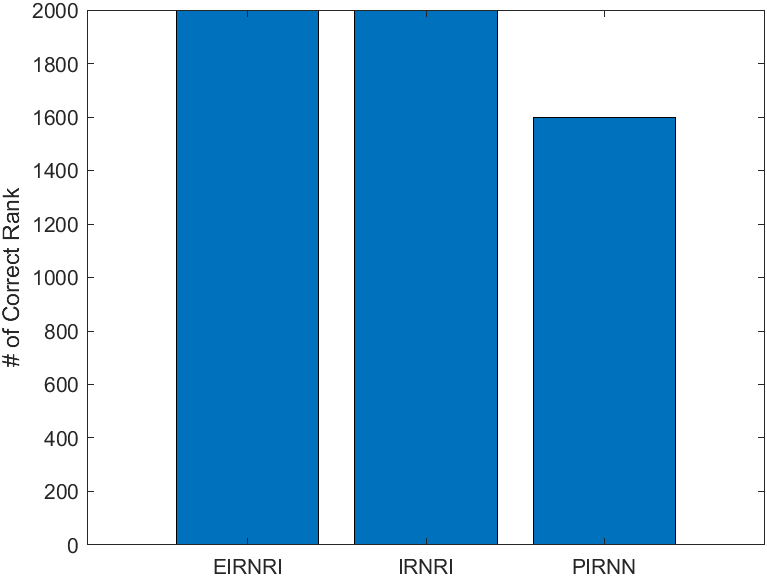
\includegraphics[width=0.3\linewidth]{Robust_rankR15_s5.png}
%   }
%   \subfigure[The number of CLD with ${\rm rank}(X^{*})=10$.]{
%       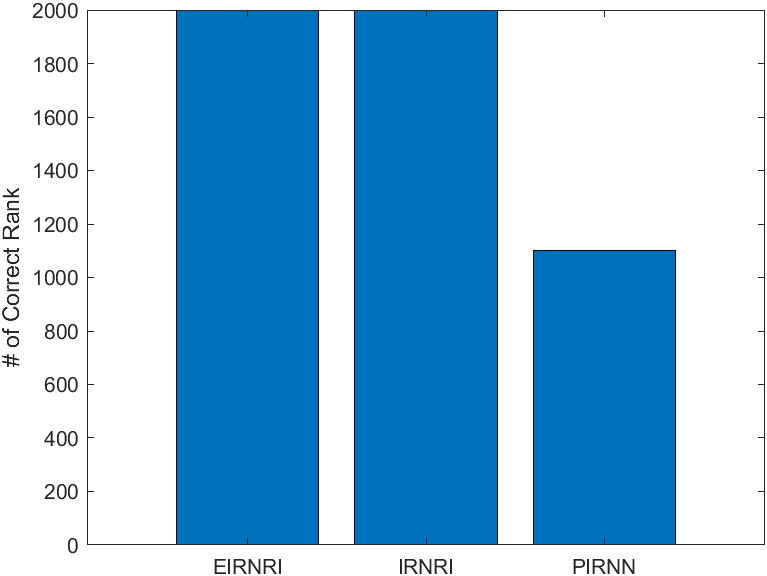
\includegraphics[width=0.3\linewidth]{Robust_rankR15_s10.png}
%   }
%   \subfigure[The number of CLD with ${\rm rank}(X^{*})=15$.]{
%       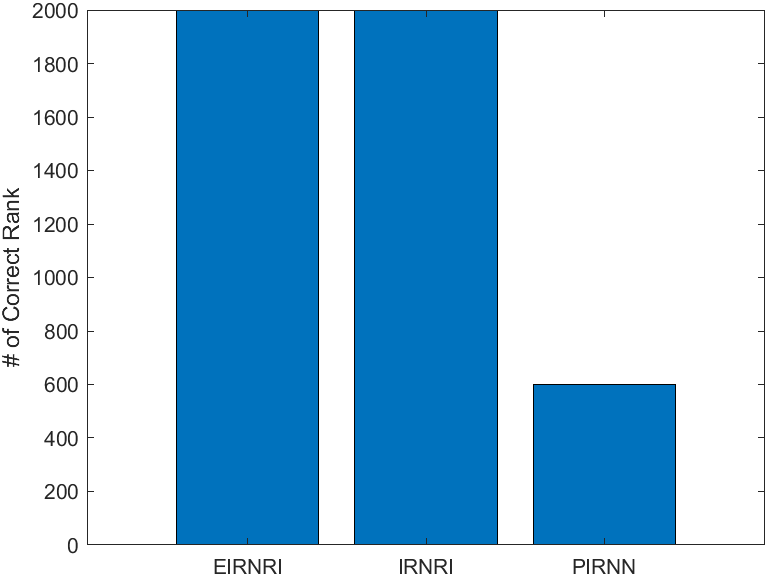
\includegraphics[width=0.3\linewidth]{Robust_rankR15_s15.png}
%   }
% }
% \captionsetup{singlelinecheck=off, justification=raggedright}
% \caption{The number of problems that achieve model identification for different ${\rm rank}(X^{*})$. For each ${\rm rank}(X^{*})$, 2000 problems are generated and set $\lambda = 10^{-1}\|X^{*}\|_{\infty}$ for those problems. We set different $\epsilon = \{10^{-1}, 10^{-2},10^{-3}\}$ for PIRNN and the default values for our algorithm.}
% \label{fig_MatrixIden}
% \end{figure}



To compare the efficiency of the algorithms,  we also plot the evolution of the relative error for each case in Figure \ref{fig.???}.  
We can see that the proposed IRNRI achieves roughly the same speed as PIRNN, while the proposed  EIRNRI 
significantly outperforms PIRNN.  
 
 % end .... 
 
 
 
 
 
 \begin{figure}[H]
  \centering{
    % \includegraphics[width=0.9\linewidth]{LLCvgc.png}
  \subfigure[${\rm rank}(X*)=5$]{
    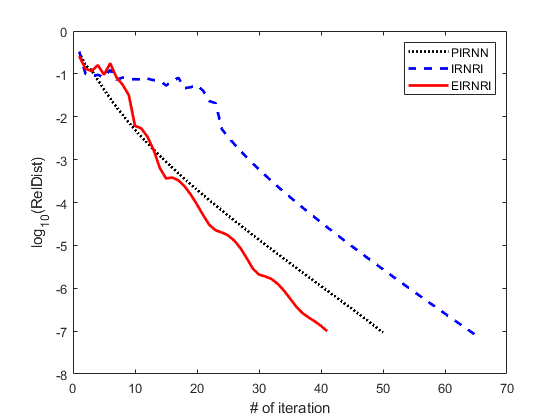
\includegraphics[width=0.3\linewidth]{randRec_InitR5_Rank5.png}
  }
  \subfigure[${\rm rank}(X*)=10$]{
      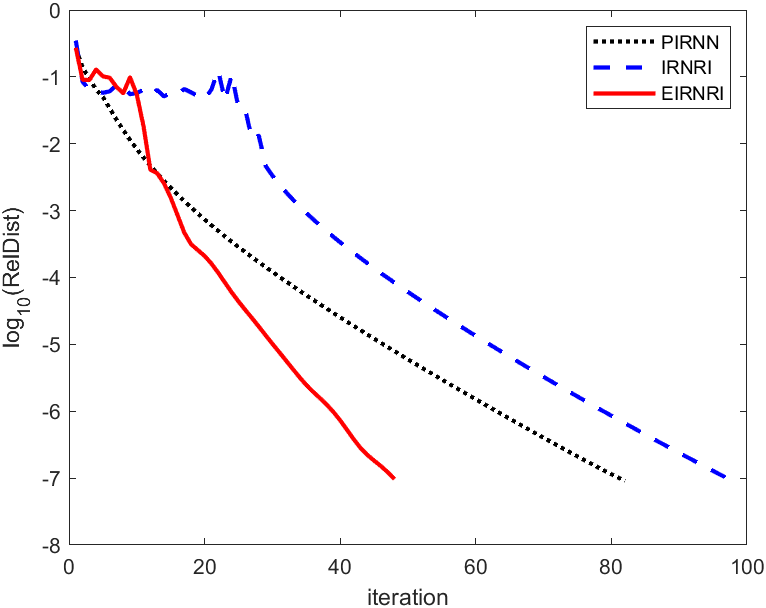
\includegraphics[width=0.3\linewidth]{randRec_InitR10_Rank10.png}
  }
  \subfigure[${\rm rank}(X*)=15$]{
      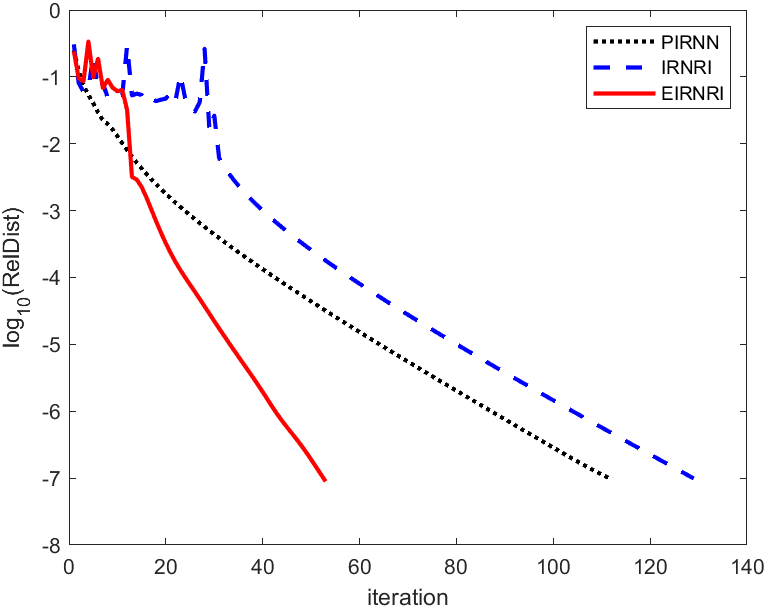
\includegraphics[width=0.3\linewidth]{randRec_InitR15_Rank15.png}
  }
}
\captionsetup{singlelinecheck=off, justification=raggedright}
\caption{Comparison of matrix recovery on synthetic data initial point with ${\rm rank}(X^{0}) = {\rm rank}(X^{*})$. We set the perturbation value to be the same for PIRNN, IRNRI, and EIRNRI at $\epsilon = 10^{-16}$, while keeping the other parameters at their default values.
% We set the same perturbation $\epsilon = 10^{-16}$ for PIRNN , AdaIRNN and EPIRNN, and set the others parameter  as default
%  value as above for other parameters. That  (a) and  (b) present the AdaIRNN performance the similar with PIRNN with, but EPIRNN obtain the optimal earlier than the above both.    
% We set a very small perturbation as, $\epsilon=10^{-8} $ for PIRNN, $\epsilon^{0} = 10^{-8}$ for AdaIRNN, EPIRNN. 
}
\label{fig_LLrate}
\end{figure}

Figure~\ref{fig_LLrate} shows IRNRI has the similar performance with PIRNN, [?]
EIRNRI has better performance than the both if the perturbation is the same.
% The algorithm has the local linear convergence rate which coincide with the results in  \cite{opt_simu_svd_2017}. 

Since Algorithm~\ref{alg_acc} introduced a new parameter $\alpha$ to accelerate the convergence, 
% and it is obviously that EIRNRI degenerate as IRNRI when $\alpha=0$,
so we set the different values of $\alpha =\{ 0,0.1,0.3,0.5,0.7,0.9\}$ to test the sensitivity to $\alpha_{k}$ for the EIRNRI algorithm. 
The experiments shows the constant momentum coefficient accelerate the convergence of the IRNRI,  and when $\alpha\approx 0.7$ EIRNRI has the best performance.
% $\alpha$ closed to $0$ or $1$   
\begin{figure}[H]
    \centering{
    \subfigure[the relative error]{
      % \includesvg{stvAlphaErr.svg}
      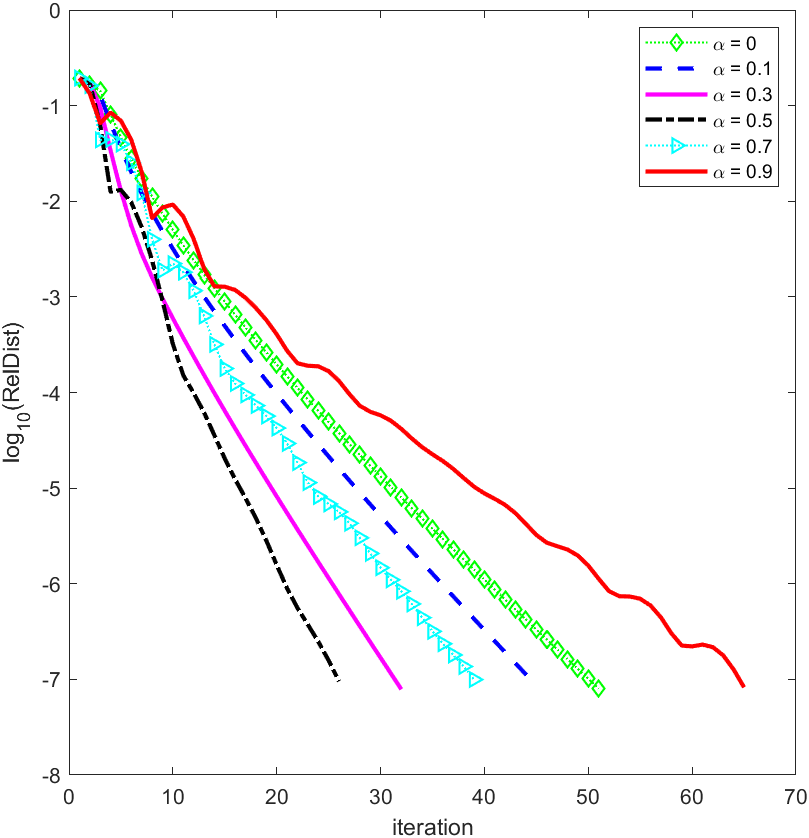
\includegraphics[width=0.3\linewidth]{stvAlpha_randRec_InitR5_Rank5.png}
    }
    \subfigure[the relative distance]{
        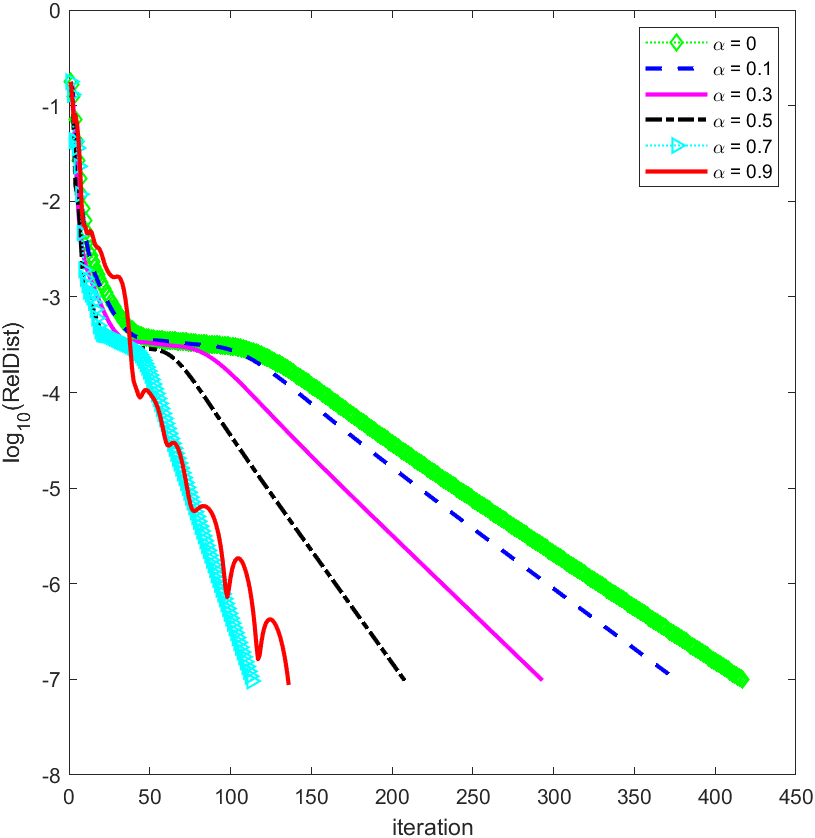
\includegraphics[width=0.3\linewidth]{stvAlpha_randRec_InitR5_Rank10.png}
    }
    \subfigure[the value of primal problem]{
        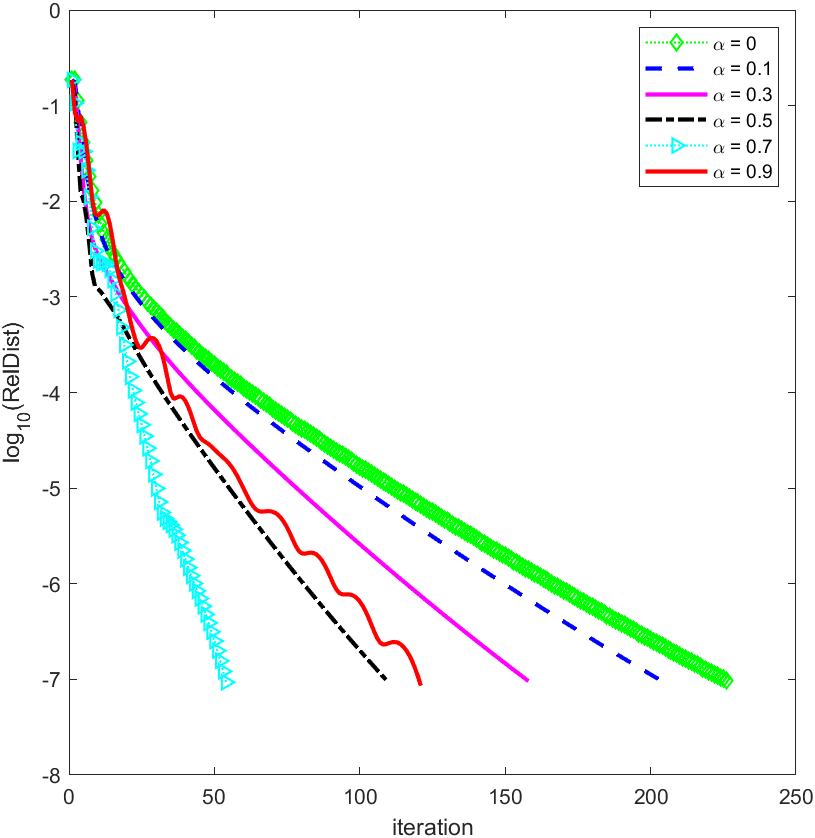
\includegraphics[width=0.3\linewidth]{stvAlpha_randRec_InitR5_Rank15.png}
    }
  }
  \captionsetup{singlelinecheck=off, justification=raggedright}
  \caption{The performance for different $\alpha$ with rank$ (X^{0})=15$, SR=$0.5$, $\mu=0.8$. It presents that $\alpha$ around $0.7$ has better performance.
  }
  \label{fig_stvAlp}
\end{figure}



\subsection{Application to Image Recovery}

% As PIRNN our algorithm is also has local linear convergence rate, and Lemma~\ref{lem_cond_cvgc_KL} shows, the AdaIRNN with warm start will local round some critical points faster, then the algorithm will convergence to the critical points.
% so AdaIRNN needs warm start when the iteration local in a new matrix set, it  coincide with the peak value of Reldist in Figure~\ref{fig_stvEPS}.
In this section, we compare  our method with three solvers, PIRNN~\cite{opt_simu_svd_2017} and Sc$p$~\cite{Relax_NCVX_CNN_RPCA_2013}\footnote{\href{https://github.com/liguorui77/scpnorm}{Available: https://github.com/liguorui77/scpnorm}
},  
FGSR$p$~\cite{LRMR_GroupSparse_2019}\footnote{\href{https://github.com/udellgroup/Codes-of-FGSR-for-effecient-low-rank-matrix-recovery}{Available: https://github.com/udellgroup/Codes-of-FGSR-for-effecient-low-rank-matrix-recovery}
}.
% {Available:github.com/liguorui77/scpnorm}
% {Available:github.com/udellgroup/Codes-of-FGSR-for-effecient-low-rank-matrix-recovery}
We consider the real images though they are usually are not low rank, but the top singular values of the real images   dominate the main information. The nature images are of scale $300 \times 300 \times 3 $, we observe the top singular value firstly, and sample the $80\% $ of the elements uniformly   for the random mask.  The other mask ????.   We set $\lambda = 1$ as the regularization parameter. 
The iteration is terminated when  $\text{RelDist}\le{10}^{-5}$ or $\text{KLopt}\le 10^{-5} $ or the number of iteration exceeds \textit{itmax}$=10^{3}$.  
We set  $\beta = 1.1$ for the three algorithms.
In order to make the PIRNN has the accurate solution we set $\epsilon = 0.0001 $ for PIRNN, then set $\epsilon^{0} = 1, \mu=0.1 $ for IRNRI and EIRNRI, set $\alpha=0.8$. 
The performance of all algorithms are compared on   two measurements  
(1)  the difference of the rank of the final iterate  and $X^{*}$,
(2) peak signal-to-noise ratio (PSNR)   



Figure \ref{fig.???} depicts ....... . 


% \cite{sp1_2021_PSNR}
\begin{equation}
  \text{PSNR} (M,X^{*}) = 10 \times \log_{10}\frac{255^{2}}{\frac{1}{3mn}\sum_{i=1}^{3}\|X_{i}^{*}-M_{i}\|_{F}^{2}}, 
\end{equation}
where $M $ is the original image and $X^{*} $ is the restored image, 
%  (2) the total iterations.  
% To compare the advantages and disadvantages of those algorithms, we use ``\textit{iter}'' to stand of the iteration cost for different algorithm.   

\begin{figure}[hbtp]
  \centering{
    \subfigure[Original]{
\includegraphics[width=0.2\linewidth]{imgRe_Lena_Rank30_Sol1_ori.png}}
    \subfigure[Low-rank image]{
\includegraphics[width=0.2\linewidth]{imgRe_Lena_Rank30_Sol2_low.png}}
    \subfigure[Random mask]{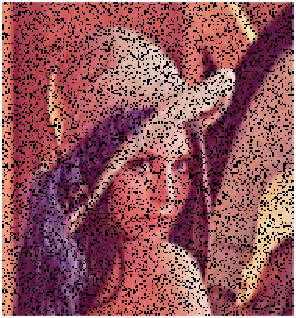
\includegraphics[width=0.2\linewidth]{imgRe_Lena_Rank30_Sol3_mask.png}}
    \subfigure[PIRNN]{
\includegraphics[width=0.2\linewidth]{imgRe_Lena_Rank30_Sol4_PIRNN.png}}
    \subfigure[AIRNN]{
\includegraphics[width=0.2\linewidth]{imgRe_Lena_Rank30_Sol5_AIRNN.png}}
    \subfigure[EIRNRI]{
\includegraphics[width=0.2\linewidth]{imgRe_Lena_Rank30_Sol6_EIRNRI.png}}
    \subfigure[Sc$p$]{
\includegraphics[width=0.2\linewidth]{imgRe_Lena_Rank30_Sol7_Scp.png}}
    \subfigure[FGSR$p$]{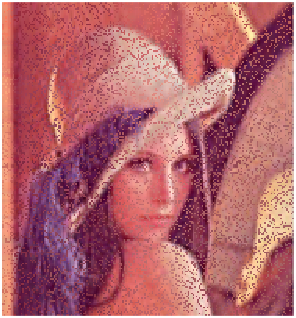
\includegraphics[width=0.2\linewidth]{imgRe_Lena_Rank30_Sol8_FGSR.png}}
  }
  \captionsetup{singlelinecheck=off, justification=raggedright}
  \caption{The performance of different methods with a random mask in image recovery with SR= $0.8$. 
    The performance for different methods with random mask in image recovery, the  
    (a) Original image, ${\rm rank}(X) = 300$; 
    (b) Low-rank image, ${\rm rank}(X^{*}) = 30$
    (c) Noised picture; 
    (d) PIRNN:  ${\rm rank}(X) = 30$,  PSNR=$28.855$;
    (e) IRNRI:  ${\rm rank}(X) = 30$,  PSNR=$28.854$;   
    (f) EIRNRI: ${\rm rank}(X) = 30$,  PSNR=$28.855$;    
    (g) Scp:    ${\rm rank}(X) = 30$,  PSNR=$28.971$;   
    (h) FGSR:   ${\rm rank}(X) = 30$,  PSNR=$21.806$;   
  }
  \label{Relimg_Lena}
\end{figure}





\begin{figure}[htbp]
  \centering{
    \subfigure[Original]{
\includegraphics[width=0.2\linewidth]{imgRe_R1_Rank30_Sol1_ori.png}}
    \subfigure[Low-rank image]{
\includegraphics[width=0.2\linewidth]{imgRe_R1_Rank30_Sol2_low.png}}
    \subfigure[Random mask]{
\includegraphics[width=0.2\linewidth]{imgRe_R1_Rank30_Sol3_mask.png}}
    \subfigure[PIRNN]{
\includegraphics[width=0.2\linewidth]{imgRe_R1_Rank30_Sol4_PIRNN.png}}
    \subfigure[AIRNN]{
\includegraphics[width=0.2\linewidth]{imgRe_R1_Rank30_Sol5_AIRNN.png}}
    \subfigure[EIRNRI]{
\includegraphics[width=0.2\linewidth]{imgRe_R1_Rank30_Sol6_EIRNRI.png}}
    \subfigure[Sc$p$]{
\includegraphics[width=0.2\linewidth]{imgRe_R1_Rank30_Sol7_Scp.png}}
    \subfigure[FGSR$p$]{
\includegraphics[width=0.2\linewidth]{imgRe_R1_Rank30_Sol8_FGSR.png}}
  }
  \captionsetup{singlelinecheck=off, justification=raggedright}
  \caption{The performance for different methods with block mask, the 
  (a) Original image, ${\rm rank}(X) = 300$; 
  (b) Low-rank image, ${\rm rank}(X^{*}) = 30$
  (c) Noised picture; 
  (d) PIRNN:  ${\rm rank}(X) = 30$,  PSNR=$28.855$;
  (e) IRNRI:  ${\rm rank}(X) = 30$,  PSNR=$28.854$;   
  (f) EIRNRI: ${\rm rank}(X) = 30$,  PSNR=$28.855$;    
  (g) Scp:    ${\rm rank}(X) = 30$,  PSNR=$28.971$;   
  (h) FGSR:   ${\rm rank}(X) = 30$,  PSNR=$21.806$;   
  }
  \label{Relimg_R1}
\end{figure}

Although Figure~\ref{Relimg_Lena} and Figure~\ref{Relimg_R1} demonstrate that all of these methods can recover the image, the iterative reweighted method appears to achieve a low-rank recovery. Scp makes the biggest PSNR in both task, but it may have a small flaw in Figure~\ref{Relimg_R1}. Since FGSR$p$ is equivalent the Schatten-$p$ norm, the parameters $\lambda$ may not appropriate in this task.
To provide more information, Table~\ref{tab_img_recovery} includes additional low-rank tasks.
% that easily obtain a low-rank solution from Table 



\begin{table}[htbp]
  \begin{tabular}{lccccccccccc}
    \toprule
                        & \multicolumn{2}{c}{PIRNN} & \multicolumn{2}{c}{IRNRI} & \multicolumn{2}{c}{EIRNRI} & \multicolumn{2}{c}{Scp} & \multicolumn{2}{c}{FGSR} \\
                        & psnr         & rank       & psnr          & rank       & psnr          & rank       & psnr        & rank      & psnr         & rank      \\
    \hline
${\rm rank}(X^{*})=15$ & 24.932       & 15         & 24.932        & 15         & 24.932        & 15         & 24.973      & 187       & 18.703       & 187       \\
${\rm rank}(X^{*})=20$ & 26.444       & 20         & 26.444        & 20         & 26.444        & 20         & 26.552      & 187       & 18.949       & 187       \\
${\rm rank}(X^{*})=25$ & 27.57        & 25         & 27.57         & 25         & 27.57         & 25         & 27.812      & 187       & 19.081       & 187       \\
${\rm rank}(X^{*})=30$ & 28.359       & 30         & 28.359        & 30         & 28.359        & 30         & 28.818      & 187       & 19.313       & 187       \\
${\rm rank}(X^{*})=35$ & 28.546       & 32         & 28.546        & 32         & 28.546        & 32         & 29.432      & 187       & 19.268       & 187       \\
${\rm rank}(X^{*})=40$ & 28.599       & 32         & 28.599        & 32         & 28.599        & 32         & 29.848      & 187       & 19.416       & 187       \\
    \bottomrule
  \end{tabular}
  \captionsetup{singlelinecheck=off, justification=raggedright}
  \caption{The performance for different mmethod with different low-rank target, bold values correspond to the best results for each algorithm. It presents that the proper perturbation affecting the algorithm less, A bigger $\epsilon$ makes PIRNN converge slower, a too small $\epsilon$ may make PIRNN get a terrible solution. The experiment shows IRNRI and EIRNRI are more robust than PIRNN when the perturbation bigger than $10^{-4}$.}
  \label{tab_img_recovery}
  \end{table}

%
%
%
%
%
%
%

% It can be seen that, all the three algorithm has the good performance on this task as they have the same PSNR, but notice that EPIRNN get the optimal solution with the least iterations. From the figure~\ref{Relimg_rank} we know that AdaIRNN and EPIRNN start form a full rank matrix while PIRNN start from the rank more close the optimal solution.  
% \begin{figure}[H]
%   \centering{
%     \subfigure[image channel 1]{\includegraphics[width=0.3\linewidth]{Relimg_rank_ch1.png}}
%     \subfigure[image channel 2]{\includegraphics[width=0.3\linewidth]{Relimg_rank_ch2.png}}
%     \subfigure[image channel 3]{\includegraphics[width=0.3\linewidth]{Relimg_rank_ch3.png}}
%   }
%   \captionsetup{singlelinecheck=off, justification=raggedright}
%   \caption{The rank with iterations}
%   \label{Relimg_rank}
% \end{figure}





\section{Conclusion and Future Work}
In this paper, we proposed, analyzed and implemented iteratively reweighted Nuclear norm methods 
for solving the Schatten-$p$ norm regularized low-rank optimization. 
Therefore two main novel features of our work.   The first is the 
rank identification property possessed by the proposed methods, meaning the algorithm can find the 
correct rank in finite iterations.  We believe this is the first work of 
pointing out the model identification property (a famous property in vector optimization) in 
matrix optimization.  Based on this property,  we also designed a novel updating strategy 
for $\epsilon_i$ to smooth the Schatten-$p$ norm, so that $\epsilon_i$ associated with the positive 
singular values can be driven to 0 rapidly and those associated with the 0 singular values can be 
automatically  fixed  as constants after finite iterations. The crucial role of this strategy is that the algorithm 
eventually behaves like a truncated weighted Nuclear norm method, so that the techniques for smooth 
algorithms can directly applied including acceleration techniques and convergence analysis. 

The convergence properties that we have proved for our algorithm were illustrated empirically on 
test sets of synthetic and real data sets. We remark, however, that many remaining practical issues 
 can be resolved to further improve the performance of the proposed method.  For example,  
 one can incorporate the rank identification property into the implementation. Since the correct 
 rank has been detected after finite iterations, the algorithm can be terminated and switch to a 
 traditional Frobenius recovery with fixed rank to further improve the quality of the recovered solution. 
 We would like leave it to the further work. 

% % % % % % % % % % % % % % % % % % % % % % % % %
% \newpage
% \blindmathpaper

% Here is a citation \cite{chow:68}.

% Acknowledgements and Disclosure of Funding should go at the end, before appendices and references

\acks{ We would like to acknowledge the support for this paper from the and the Natural Science Foundation of Shanghai under Grant 21ZR1442800 and the Young Scientists Fund of the National Natural Science Foundation of China No. 12001367.}

% Manual newpage inserted to improve layout of sample file - not
% needed in general before appendices/bibliography.



% % % % % % % % % % % % % % % % % % % % % % % % %
% \newpage
% \appendix
% \section{}
% \label{app:theorem}

% % Note: in this sample, the section number is hard-coded in. Following
% % proper LaTeX conventions, it should properly be coded as a reference:

% %In this appendix we prove the following theorem from
% %Section~\ref{sec:textree-generalization}:
% In this appendix we prove the following theorem from
% Section~6.2:
% \noindent
% {\bf Theorem} {\it Let $u,v,w$ be discrete variables such that $v, w$ do
% not co-occur with $u$ (i.e., $u\neq0\;\Rightarrow \;v=w=0$ in a given
% dataset $\dataset$). Let $N_{v0},N_{w0}$ be the number of data points for
% which $v=0, w=0$ respectively, and let $I_{uv},I_{uw}$ be the
% respective empirical mutual information values based on the sample
% $\dataset$. Then
% \[
% 	N_{v0} \;>\; N_{w0}\;\;\Rightarrow\;\;I_{uv} \;\leq\;I_{uw}
% \]
% with equality only if $u$ is identically 0.} \hfill\BlackBox

% \section{}
% \noindent
% {\bf Proof}. We use the notation:
% \[
% P_v(i) \;=\;\frac{N_v^i}{N},\;\;\;i \neq 0;\;\;\;
% P_{v0}\;\equiv\;P_v(0)\; = \;1 - \sum_{i\neq 0}P_v(i).
% \]
% These values represent the (empirical) probabilities of $v$
% taking value $i\neq 0$ and 0 respectively.  Entropies will be denoted
% by $H$. We aim to show that $\fracpartial{I_{uv}}{P_{v0}} < 0$....\\
% {\noindent \em Remainder omitted in this sample. See http://www.jmlr.org/papers/ for full paper.}


\vskip 0.2in
\bibliography{sample}

\end{document}
